\documentclass{beamer}

%%% paquetes
\usepackage[spanish]{babel}
\usepackage{amsmath, amsthm, amssymb}
\usepackage{mathtools}
\usepackage{verbatim}
\usepackage{tikz}
\usepackage{graphics}
\usepackage{ulem}
\usepackage{enumitem}
\DeclareUnicodeCharacter{2260}{$\neq$}
% DEFINICIÓN DE COMANDOS Y ENTORNOS

% CONJUNTOS DE NÚMEROS
  \newcommand{\N}{\mathbb{N}}     % Naturales
  \newcommand{\R}{\mathbb{R}}     % Reales
  \newcommand{\Z}{\mathbb{Z}}     % Enteros
  \newcommand{\Q}{\mathbb{Q}}     % Racionales
  \newcommand{\C}{\mathbb{C}}     % Complejos

% Otros comandos propios
  \newcommand{\mun}{\{\mu_n\}_{n \in \N_0}}                  				        % Sucesión de momentos
  \newcommand{\pol}{\mathbb{P}[x]}                           				        % Polinomios
  \newcommand{\funl}{\mathcal{L}}                            				        % Funcional de momentos L
  \newcommand{\spol}{\{P_n\}_{n \in \N_0}}                   				        % Sucesión de polinomios
  \newcommand{\pescalar}[2]{\langle #1, #2 \rangle}      				            % Producto escalar
  \newcommand{\charlier}{\{C_n^{(\mu)}\}_{n \in \N_0}}       			   	      % SPOVD de Charlier
  \newcommand{\meixner}{\{M_n^{(\beta, c)}\}_{n \in \N_0}}                 	% SPOVD de Meixner
  \newcommand{\kraw}{\{K_n^{(p)}\}_{n \in \{0, \dots, N-1\}}}              	% SPOVD de Krawtchouk
  \newcommand{\hahn}{\{h_n^{(\alpha, \beta)}\}_{n \in \{0, \dots, N-1\}}}	  % SPOVD de Hahn
  \newcommand{\eprob}{(\Omega, \mathcal A, P)}              				        % Espacio de probabilidad
  \newcommand{\pest}{\{X_t\}_{t \in T}}                     				        % Proceso estocástico
  \newcommand{\markov}{\{X_t\}_{t \in \mathbb{N}_0}}        				        % Cadena de Markov
  \newcommand{\pnm}{\{X_t\}_{t \in [0, \infty[}}            				        % Proceso de nacimiento y muerte

% Para escalar matemáticas:
  \newcommand{\scalemath}[2]{\scalebox{#1}{\mbox{\ensuremath{\displaystyle #2}}}}

% TEOREMAS Y ENTORNOS ASOCIADOS

  % \newtheorem{theorem}{Theorem}[chapter]
  \newtheorem*{teorema*}{Teorema}
  \newtheorem{teorema}{Teorema}[chapter]
  \newtheorem{proposicion}[teorema]{Proposición}
  \newtheorem{lema}[teorema]{Lema}
  \newtheorem{corolario}[teorema]{Corolario}

    \theoremstyle{definition}
  \newtheorem{definicion}[teorema]{Definición}
  \newtheorem{ejemplo}[teorema]{Ejemplo}

    \theoremstyle{remark}
  \newtheorem{observacion}[teorema]{Observación}


%%% Tema
\usetheme{Madrid}
\usecolortheme{beaver}

%%% Portada
\title[TFG] %optional
{Criptosistemas basados en el \\ problema de la mochila}
\subtitle{Trabajo Fin de Grado del \\ Doble Grado en Ingeniería Informática y Matemáticas}
\author[Juan Manuel Mateos Pérez] % (optional, for multiple authors)
{Juan Manuel Mateos Pérez}
\institute[UGR] % (optional)
{
    Universidad de Granada \\
    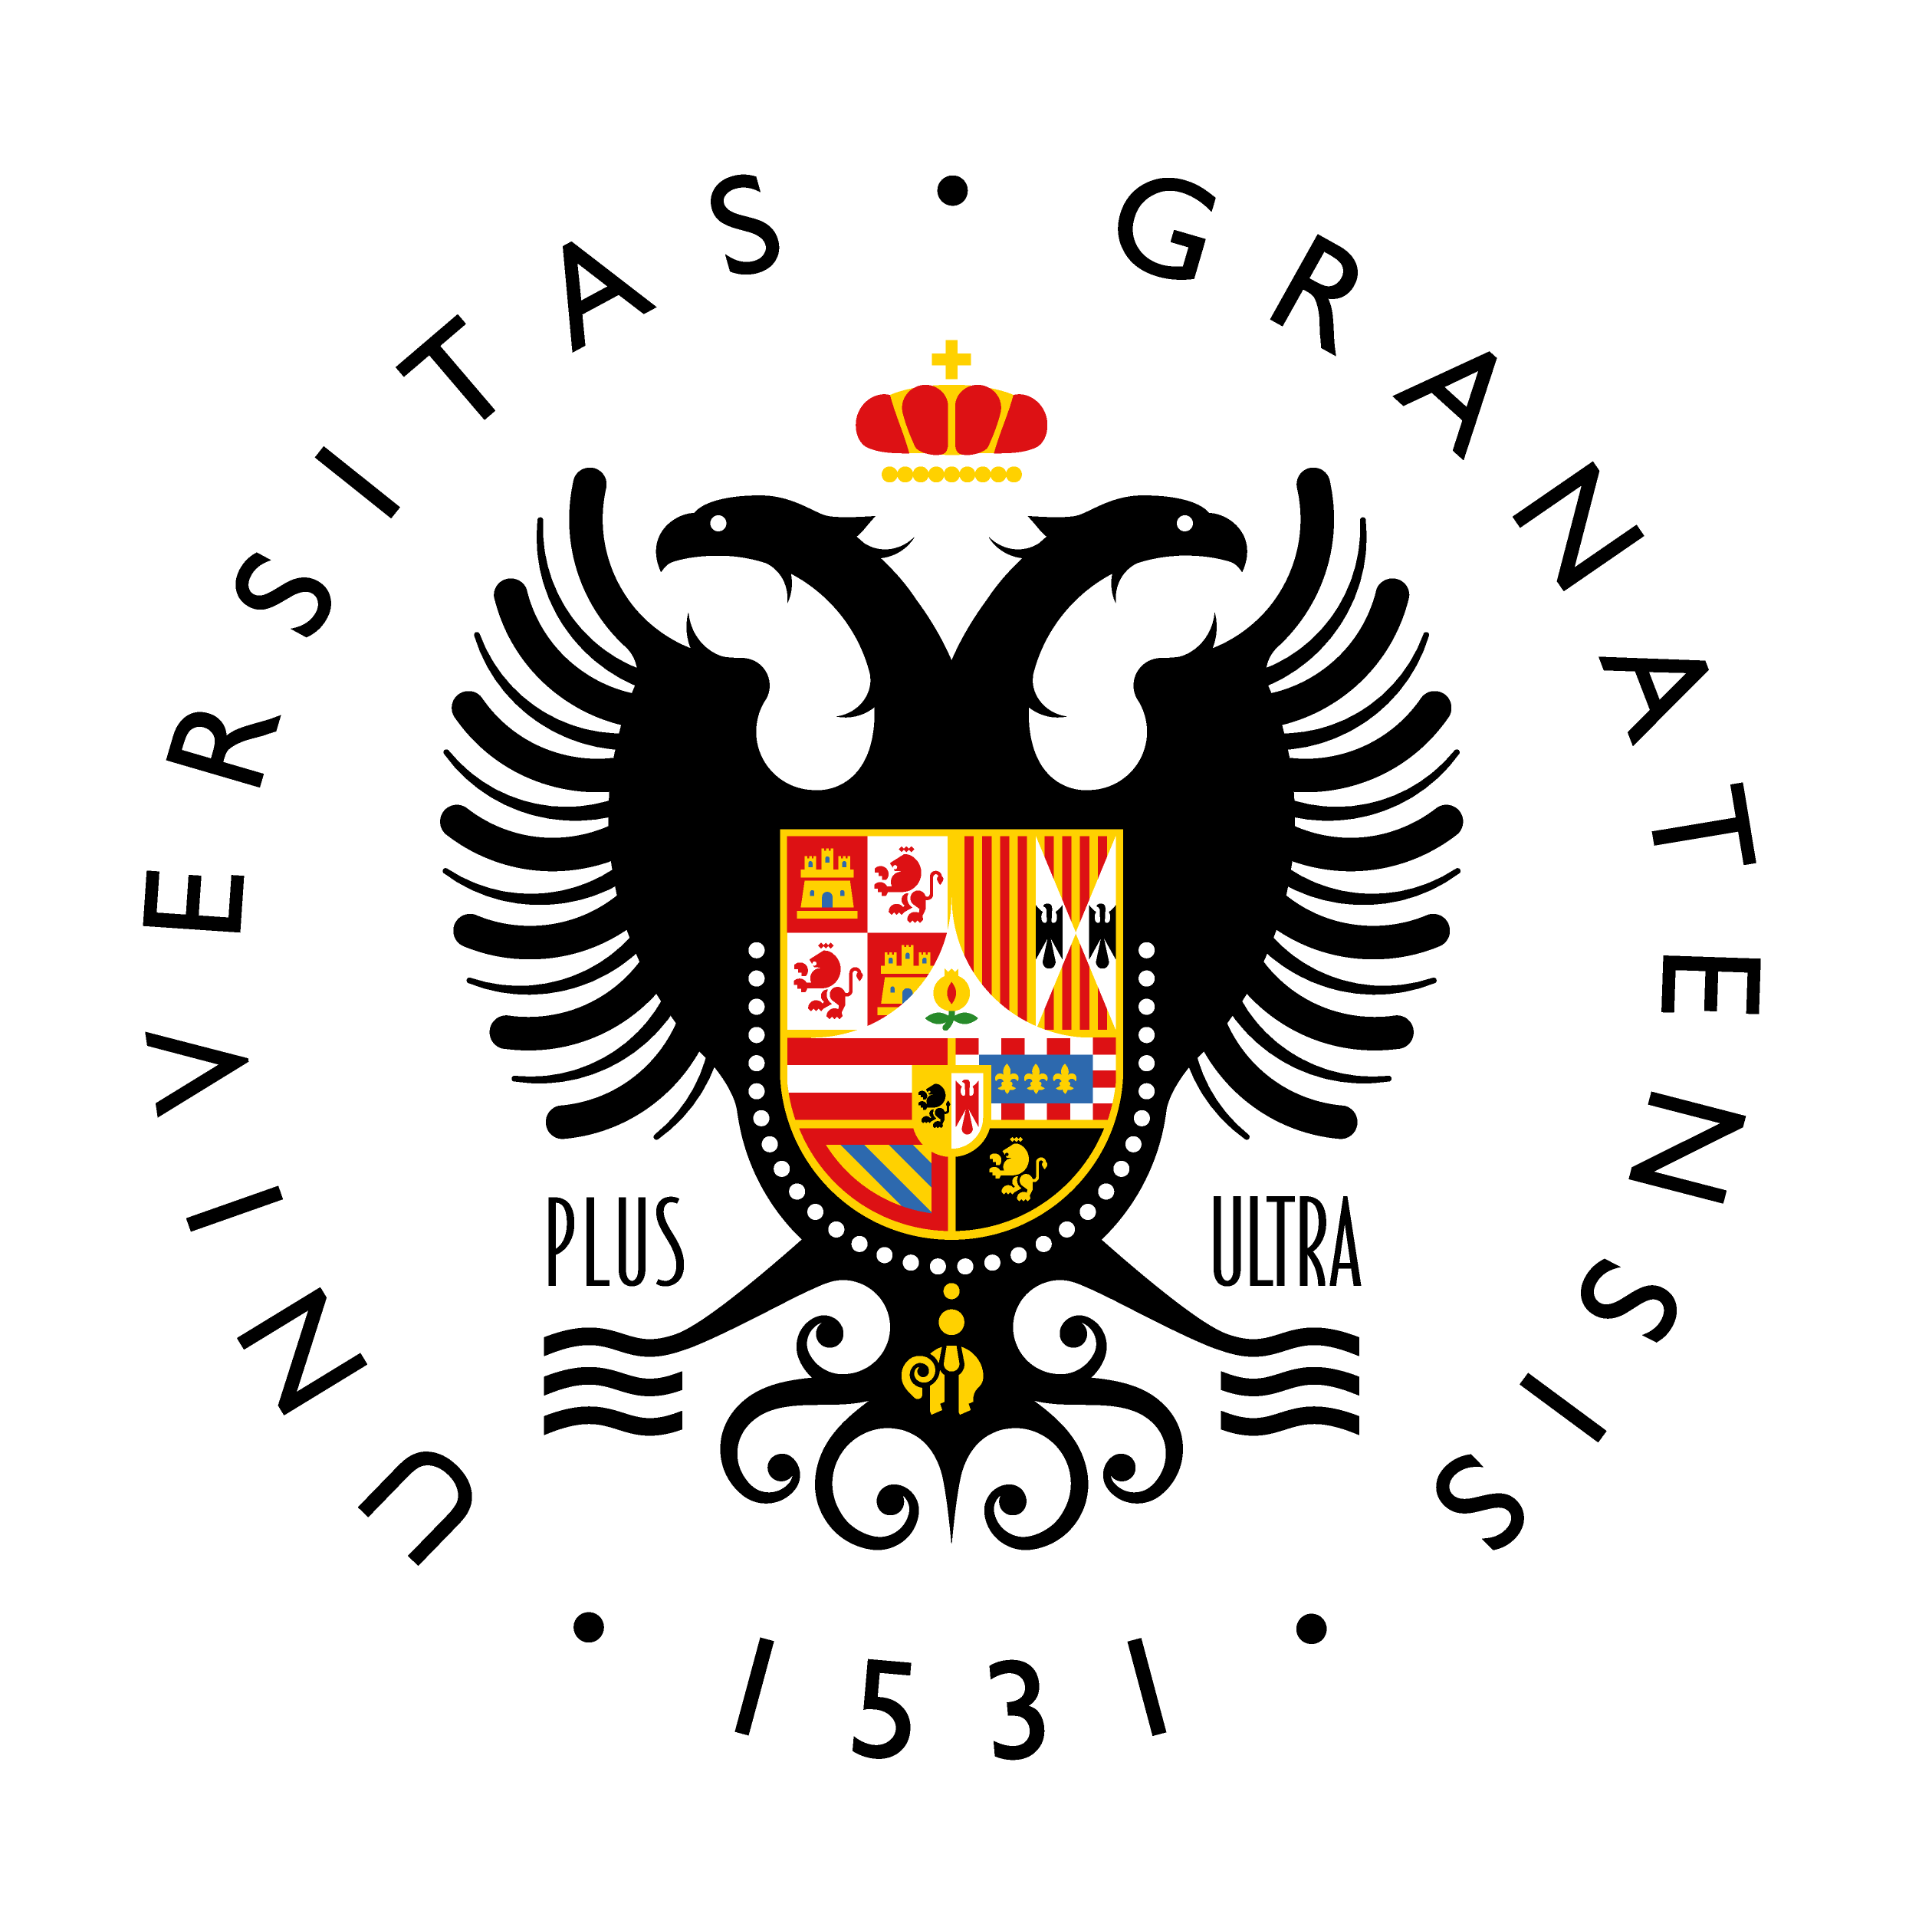
\includegraphics[width=2cm]{img/ugr.png}
}
\date[Curso 2023-2024] % (optional)
{Curso 2023-2024}

%%% Índice al inicio de sección
\AtBeginSection[]
{
  \begin{frame}
    \frametitle{Tabla de contenidos}
    \tableofcontents[currentsection]
  \end{frame}
}

%%%% Inicio del documento
\begin{document}
    
    % Título
    \begin{frame}
        \titlepage
    \end{frame}

    % Objetivos
    \begin{frame}{Objetivos}
        \begin{itemize}
            \item Compresión del problema de la mochila.
            \item Análisis de los criptosistemas de Merkle-Hellman y Chor-Rivest.
            \item Estudio de los ataques de Shamir, Lagarias-Odlyzko y Coster et al. 
        \end{itemize}
    \end{frame}

    % Índice
    \begin{frame}
        \frametitle{Tabla de contenidos}
        \tableofcontents
    \end{frame}

    % Criptografía Básica
    \section{Criptografía básica}
    \subsection{Introducción a la criptografía}

        \begin{frame}{Criptografía}
            \begin{block}{Definición}
                La criptografía (del griego kryptós, «secreto», y graphé, «grafo», literalmente «escritura secreta») es una disciplina que se ocupa de la seguridad de la información en la comunicación a través de canales inseguros.
            \end{block}
        \end{frame}
    
        \begin{frame}{Historia de la criptografía}
            \begin{columns}
                \column{0.35\textwidth}
                \begin{flushright}
                    \vspace{0.6cm}
                    $600$ a.C.
                    \vspace{3.5cm} \\
                    $5$ a.C.
                \end{flushright}
                
                \column{0.3\textwidth}
                \begin{figure}
                    \centering
                    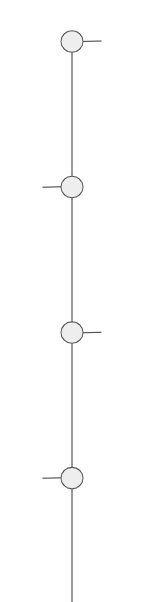
\includegraphics[width=0.5\linewidth, height=0.9\textheight]{img/Eje_cronologico.png}
                \end{figure}

                \column{0.35\textwidth}
                \begin{flushleft}
                    \vspace{-0.3cm}
                    $2500$ a.C.
                    \vspace{3.5cm} \\
                    $50$ a.C.
                    \vspace{3cm}
                \end{flushleft}
            \end{columns}
        \end{frame}

        \begin{frame}{Historia de la criptografía}
            \begin{columns}
                \column{0.35\textwidth}
                \begin{flushright}
                    \vspace{0.6cm}
                    $600$ a.C.
                    \vspace{3.5cm} \\
                    $5$ a.C.
                \end{flushright}
                
                \column{0.3\textwidth}
                \begin{figure}
                    \centering
                    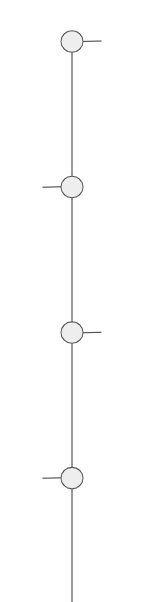
\includegraphics[width=0.5\linewidth, height=0.9\textheight]{img/Eje_cronologico.png}
                \end{figure}

                \column{0.35\textwidth}
                \begin{flushleft}
                    \vspace{-0.3cm}
                    \textbf{Egipcios}, $2500$ a.C.
                    \vspace{3.5cm} \\
                    $50$ a.C.
                    \vspace{3cm}
                \end{flushleft}
            \end{columns}
        \end{frame}
        
        \begin{frame}{Historia de la criptografía}
            \begin{columns}
                \column{0.35\textwidth}
                \begin{flushright}
                    \vspace{0.6cm}
                    \textbf{Hebreos}, $600$ a.C.
                    \vspace{3.5cm} \\
                    $5$ a.C.
                \end{flushright}
                
                \column{0.3\textwidth}
                \begin{figure}
                    \centering
                    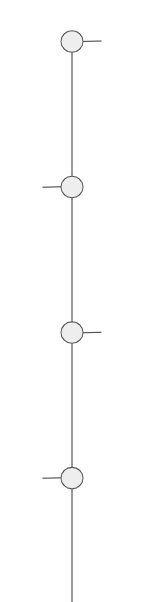
\includegraphics[width=0.5\linewidth, height=0.9\textheight]{img/Eje_cronologico.png}
                \end{figure}

                \column{0.35\textwidth}
                \begin{flushleft}
                    \vspace{-0.3cm}
                    Egipcios, $2500$ a.C.
                    \vspace{3.5cm} \\
                    $50$ a.C.
                    \vspace{3cm}
                \end{flushleft}
            \end{columns}
        \end{frame}

        \begin{frame}{Historia de la criptografía}
            \begin{columns}
                \column{0.35\textwidth}
                \begin{flushright}
                    \vspace{0.6cm}
                    Hebreos, $600$ a.C.
                    \vspace{3.5cm} \\
                    $5$ a.C.
                \end{flushright}
                
                \column{0.3\textwidth}
                \begin{figure}
                    \centering
                    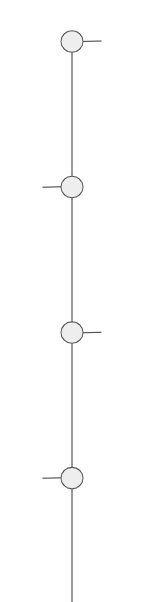
\includegraphics[width=0.5\linewidth, height=0.9\textheight]{img/Eje_cronologico.png}
                \end{figure}

                \column{0.35\textwidth}
                \begin{flushleft}
                    \vspace{-0.3cm}
                    Egipcios, $2500$ a.C.
                    \vspace{3.5cm} \\
                    \textbf{Romanos}, $50$ a.C.
                    \vspace{3cm}
                \end{flushleft}
            \end{columns}
        \end{frame}

        \begin{frame}{Historia de la criptografía}
            \begin{columns}
                \column{0.35\textwidth}
                \begin{flushright}
                    \vspace{0.6cm}
                    Hebreos, $600$ a.C.
                    \vspace{3.5cm} \\
                    \textbf{Griegos}, $5$ a.C.
                \end{flushright}
                
                \column{0.3\textwidth}
                \begin{figure}
                    \centering
                    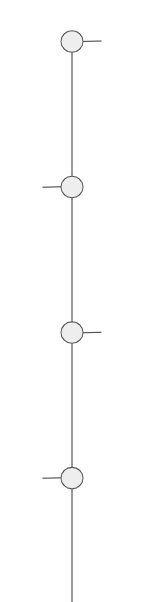
\includegraphics[width=0.5\linewidth, height=0.9\textheight]{img/Eje_cronologico.png}
                \end{figure}

                \column{0.35\textwidth}
                \begin{flushleft}
                    \vspace{-0.3cm}
                    Egipcios, $2500$ a.C.
                    \vspace{3.5cm} \\
                    Romanos, $50$ a.C.
                    \vspace{3cm}
                \end{flushleft}
            \end{columns}
        \end{frame}

        \begin{frame}{Desarrollo de la criptografía}
            \begin{columns}
                \column{0.35\textwidth}
                \begin{flushright}
                    \vspace{2cm}
                    $1976$ d.C.
                \end{flushright}
                
                \column{0.3\textwidth}
                \begin{figure}
                    \centering
                    \vspace{-2.2cm}
                    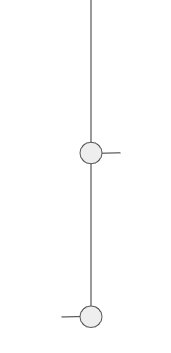
\includegraphics[width=0.6\linewidth, height=0.6\textheight]{img/Eje_cronologico2.png}
                \end{figure}

                \column{0.35\textwidth}
                \begin{flushleft}
                    \vspace{-3cm}
                    $1939$ d.C.
                \end{flushleft}
            \end{columns}
        \end{frame}

        \begin{frame}{Desarrollo de la criptografía}
            \begin{columns}
                \column{0.35\textwidth}
                \begin{flushright}
                    \vspace{2cm}
                    $1976$ d.C.
                \end{flushright}
                
                \column{0.3\textwidth}
                \begin{figure}
                    \centering
                    \vspace{-2.2cm}
                    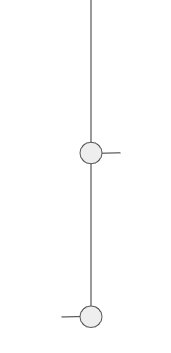
\includegraphics[width=0.6\linewidth, height=0.6\textheight]{img/Eje_cronologico2.png}
                \end{figure}

                \column{0.35\textwidth}
                \begin{flushleft}
                    \vspace{-1cm}
                    \hspace{-1cm}
                    \textbf{Segunda Guerra Mundial}, $1939$ d.C.
                    \vspace{0.5cm}
                    \hspace{-2cm}
                    \begin{itemize}
                        \item Enigma
                        \item Maquinas de Turing 
                    \end{itemize}
                \end{flushleft}
            \end{columns}
        \end{frame}

        \begin{frame}{Desarrollo de la criptografía}
            \begin{columns}
                \column{0.35\textwidth}
                \begin{flushright}
                    \vspace{3.2cm}
                    \textbf{Diffie-Hellman}, \\ $1976$ d.C.
                    \vspace{0.5cm}
                \end{flushright}
                
                \column{0.3\textwidth}
                \begin{figure}
                    \centering
                    \vspace{-1.5cm}
                    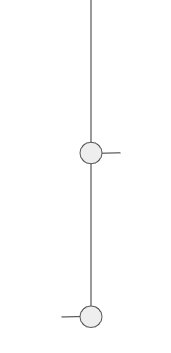
\includegraphics[width=0.6\linewidth, height=0.6\textheight]{img/Eje_cronologico2.png}
                \end{figure}

                \column{0.35\textwidth}
                \begin{flushleft}
                    \vspace{-2.3cm}
                    \hspace{-1cm}
                    Segunda Guerra Mundial, \\ $1939$ d.C.
                \end{flushleft}
            \end{columns}
            \begin{itemize}
                \item Criptografía simétrica
                \item Criptografía asimétrica
            \end{itemize}
        \end{frame}

    \subsection{Criptografía simétrica vs asimétrica}
        
        \begin{frame}{Criptografía simétrica vs asimétrica}
            \begin{columns}
                \column{0.45\textwidth}
                \centering
                \uline{Criptografía simétrica}
                \\ \vspace{0.5cm}
                \begin{itemize}
                    \item Clave única (necesidad de compartirla)
                    \item Más velocidad
                    \item No se necesita comprobar autenticación
                \end{itemize}

                \column{0.1\textwidth}
                \centering
                \vspace{3cm}
                vs

                \column{0.45\textwidth}
                \centering
                \uline{Criptografía asimétrica}
                \\ \vspace{0.5cm}
                \begin{itemize}
                    \item Dos claves por usuario (existencia de clave pública)
                    \item Menos velocidad
                    \item Se necesita comprobar autenticación
                \end{itemize}
            \end{columns}
        \end{frame}

        \begin{frame}{Criptografía simétrica vs asimétrica}
            \begin{columns}
                \column{0.45\textwidth}
                \centering
                \textbf{\uline{Criptografía simétrica}}
                \\ \vspace{0.5cm}
                \begin{itemize}
                    \item \textbf{Clave única (necesidad de compartirla)}
                    \item \textbf{Más velocidad}
                    \item \textbf{No se necesita comprobar autenticación}
                \end{itemize}

                \column{0.1\textwidth}
                \centering
                \vspace{3cm}
                vs

                \column{0.45\textwidth}
                \centering
                \uline{Criptografía asimétrica}
                \\ \vspace{0.5cm}
                \begin{itemize}
                    \item Dos claves por usuario (existencia de clave pública)
                    \item Menos velocidad
                    \item Se necesita comprobar autenticación
                \end{itemize}
            \end{columns}
        \end{frame}

        \begin{frame}{Cifrado simétrico}
            \begin{columns}
                \column{0.33\textwidth}
                \centering
                \begin{figure}
                    \vspace{1.75cm}
                    
\includegraphics[width=0.5\linewidth]{img/Personaje_izquierda.png}
                    \\
                    \text{Alice}
                \end{figure}

                \column{0.33\textwidth}
                \centering
                \vspace{3.1cm}
                \begin{figure}
                    
\includegraphics[width=0.9\linewidth, height=0.15\textheight]{img/flecha_derecha.png}
                    \\
                    \text{$mensaje$}
                \end{figure}
            
                \column{0.33\textwidth}
                \centering
                \begin{figure}
                    \vspace{1.8cm}
                    
\includegraphics[width=0.5\linewidth]{img/Personaje_derecha.png}
                    \\
                    \text{Bob}
                \end{figure}
            \end{columns}
        \end{frame}

        \begin{frame}{Cifrado simétrico}
            \begin{columns}
                \column{0.33\textwidth}
                \centering
                \begin{figure}
                    \vspace{1.75cm}
                    
\includegraphics[width=0.5\linewidth]{img/Personaje_izquierda.png}
                    \\
                    \text{Alice}
                \end{figure}

                \column{0.33\textwidth}
                \centering
                \begin{figure}
                    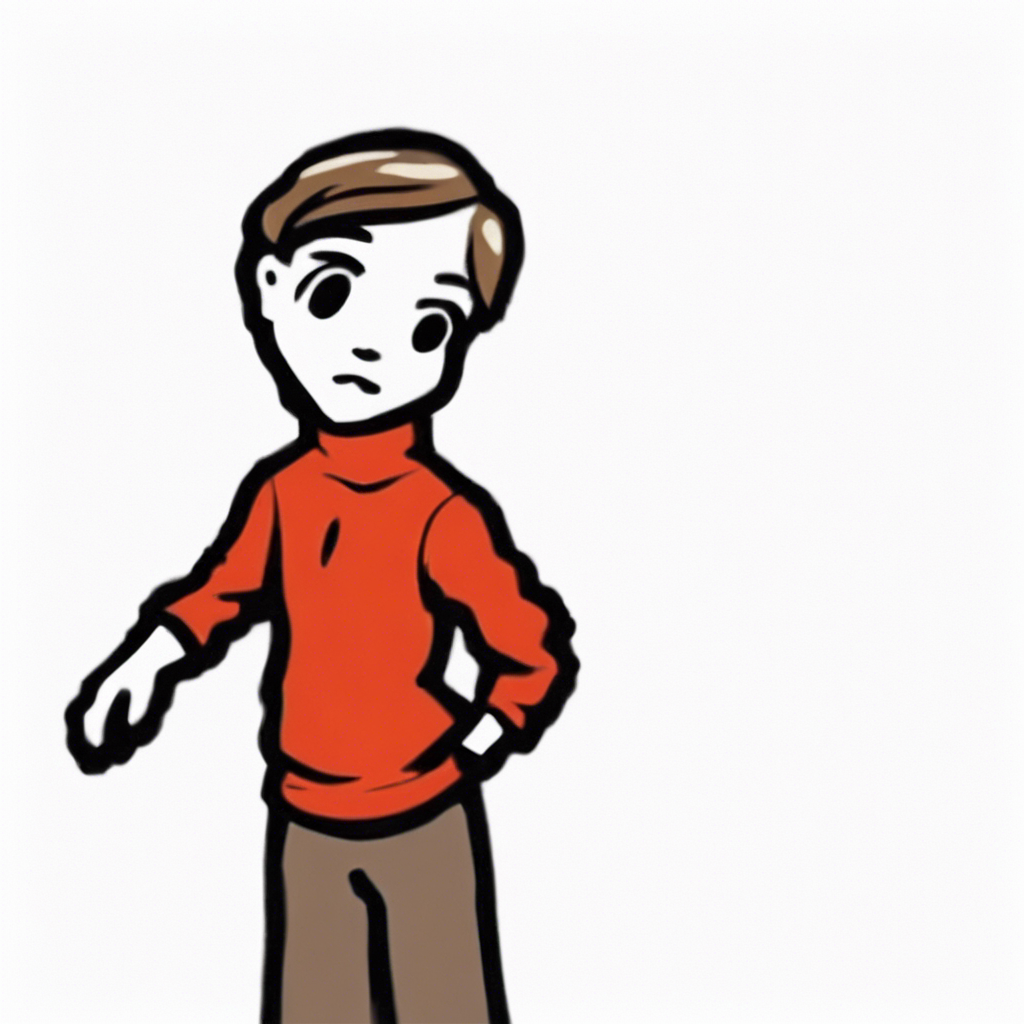
\includegraphics[width=0.5\linewidth]{img/Eva.png}
                    \\
                    \text{$Eva$}
                \end{figure}
                \begin{figure}
                    
\includegraphics[width=0.9\linewidth, height=0.15\textheight]{img/flecha_derecha.png}
                    \\
                    \text{$mensaje$}
                \end{figure}
            
                \column{0.33\textwidth}
                \centering
                \begin{figure}
                    \vspace{1.8cm}
                    
\includegraphics[width=0.5\linewidth]{img/Personaje_derecha.png}
                    \\
                    \text{Bob}
                \end{figure}
            \end{columns}
        \end{frame}

        \begin{frame}{Cifrado simétrico}
            \begin{columns}
                \column{0.33\textwidth}
                \centering
                \begin{figure}
                    \text{$enc_{k}(mensaje) = x$}
                    \\
                    \vspace{0.25cm}
                    
\includegraphics[width=0.2\linewidth, height=0.1\textheight]{img/flecha_misma.png}
                    \\
                    
\includegraphics[width=0.5\linewidth]{img/Personaje_izquierda.png}
                    \\
                    \text{Alice}
                \end{figure}

                \column{0.33\textwidth}
                \centering
                \begin{figure}
                    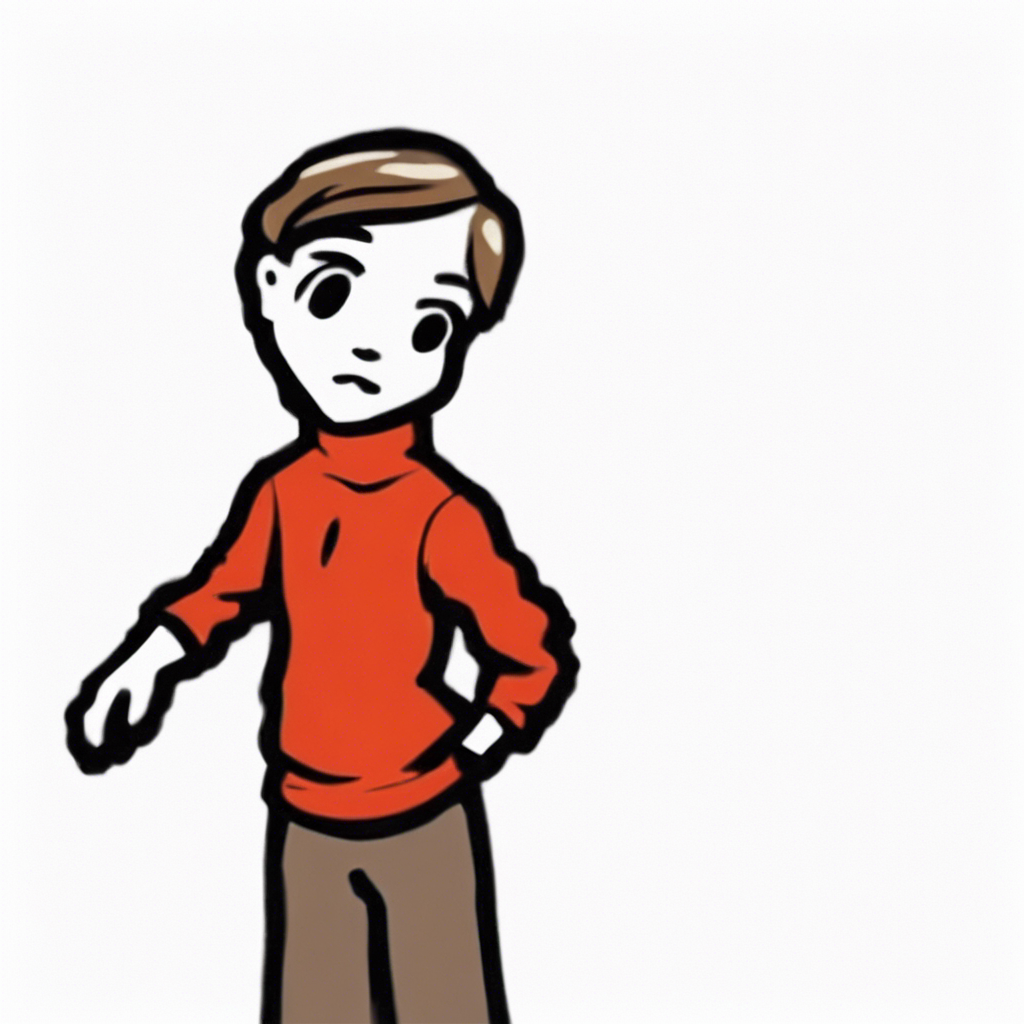
\includegraphics[width=0.5\linewidth]{img/Eva.png}
                    \\
                    \text{$Eva$}
                \end{figure}
                \begin{figure}
                    
\includegraphics[width=0.9\linewidth, height=0.15\textheight]{img/flecha_derecha.png}
                    \\
                    \text{$x$}
                \end{figure}
            
                \column{0.33\textwidth}
                \centering
                \begin{figure}
                    \vspace{1.8cm}
                    
\includegraphics[width=0.5\linewidth]{img/Personaje_derecha.png}
                    \\
                    \text{Bob}
                \end{figure}
            \end{columns}
        \end{frame}

        \begin{frame}{Cifrado simétrico}
            \begin{columns}
                \column{0.33\textwidth}
                \centering
                \begin{figure}
                    \text{$enc_{k}(mensaje) = x$}
                    \\
                    \vspace{0.25cm}
                    
\includegraphics[width=0.2\linewidth, height=0.1\textheight]{img/flecha_misma.png}
                    \\
                    
\includegraphics[width=0.5\linewidth]{img/Personaje_izquierda.png}
                    \\
                    \text{Alice}
                \end{figure}

                \column{0.33\textwidth}
                \centering
                \begin{figure}
                    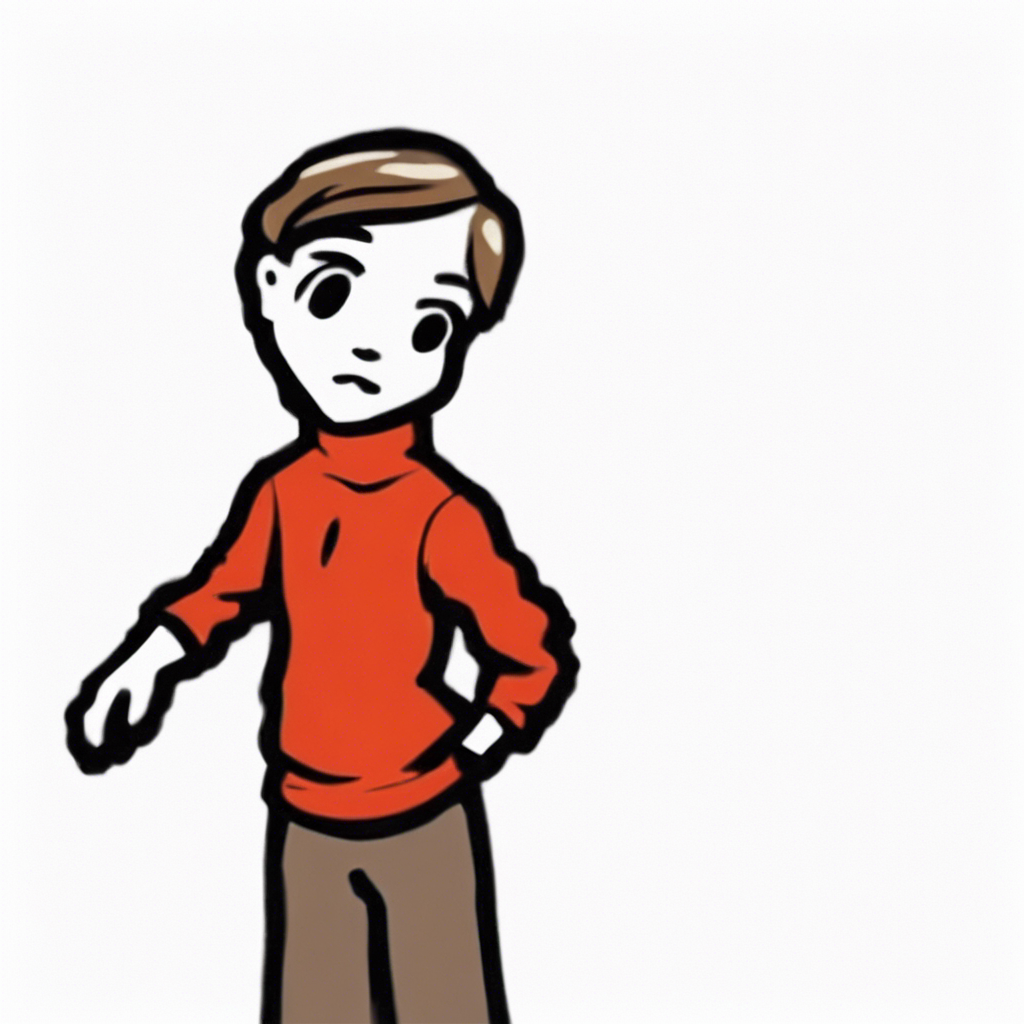
\includegraphics[width=0.5\linewidth]{img/Eva.png}
                    \\
                    \text{$Eva$}
                \end{figure}
                \begin{figure}
                    
\includegraphics[width=0.9\linewidth, height=0.15\textheight]{img/flecha_derecha.png}
                    \\
                    \text{$x$}
                \end{figure}
            
                \column{0.33\textwidth}
                \centering
                \begin{figure}
                    \text{$dec_{k}(x) = mensaje$}
                    \\
                    \vspace{0.3cm}
                    
\includegraphics[width=0.2\linewidth, height=0.1\textheight]{img/flecha_misma.png}
                    \\
                    
\includegraphics[width=0.5\linewidth]{img/Personaje_derecha.png}
                    \\
                    \text{Bob}
                \end{figure}
            \end{columns}
        \end{frame}

        \begin{frame}{Criptografía simétrica vs asimétrica}
            \begin{columns}
                \column{0.45\textwidth}
                \centering
                \uline{Criptografía simétrica}
                \\ \vspace{0.5cm}
                \begin{itemize}
                    \item Clave única (necesidad de compartirla)
                    \item Más velocidad
                    \item No se necesita comprobar autenticación
                \end{itemize}

                \column{0.1\textwidth}
                \centering
                \vspace{3cm}
                vs

                \column{0.45\textwidth}
                \centering
                \uline{Criptografía asimétrica}
                \\ \vspace{0.5cm}
                \begin{itemize}
                    \item Dos claves por usuario (existencia de clave pública)
                    \item Menos velocidad
                    \item Se necesita comprobar autenticación
                \end{itemize}
            \end{columns}
        \end{frame}

        \begin{frame}{Criptografía simétrica vs asimétrica}
            \begin{columns}
                \column{0.45\textwidth}
                \centering
                \uline{Criptografía simétrica}
                \\ \vspace{0.5cm}
                \begin{itemize}
                    \item Clave única (necesidad de compartirla)
                    \item Más velocidad
                    \item No se necesita comprobar autenticación
                \end{itemize}

                \column{0.1\textwidth}
                \centering
                \vspace{3cm}
                vs

                \column{0.45\textwidth}
                \centering
                \textbf{\uline{Criptografía asimétrica}}
                \\ \vspace{0.5cm}
                \begin{itemize}
                    \item \textbf{Dos claves por usuario (existencia de clave pública)}
                    \item \textbf{Menos velocidad}
                    \item \textbf{Se necesita comprobar autenticación}
                \end{itemize}
            \end{columns}
        \end{frame}

        \begin{frame}{Cifrado asimétrico}
            \begin{columns}
                \column{0.33\textwidth}
                \centering
                \begin{figure}
                    \vspace{1.75cm}
                    
\includegraphics[width=0.5\linewidth]{img/Personaje_izquierda.png}
                    \\
                    \text{Alice}
                \end{figure}

                \column{0.33\textwidth}
                \centering
                \begin{figure}
                    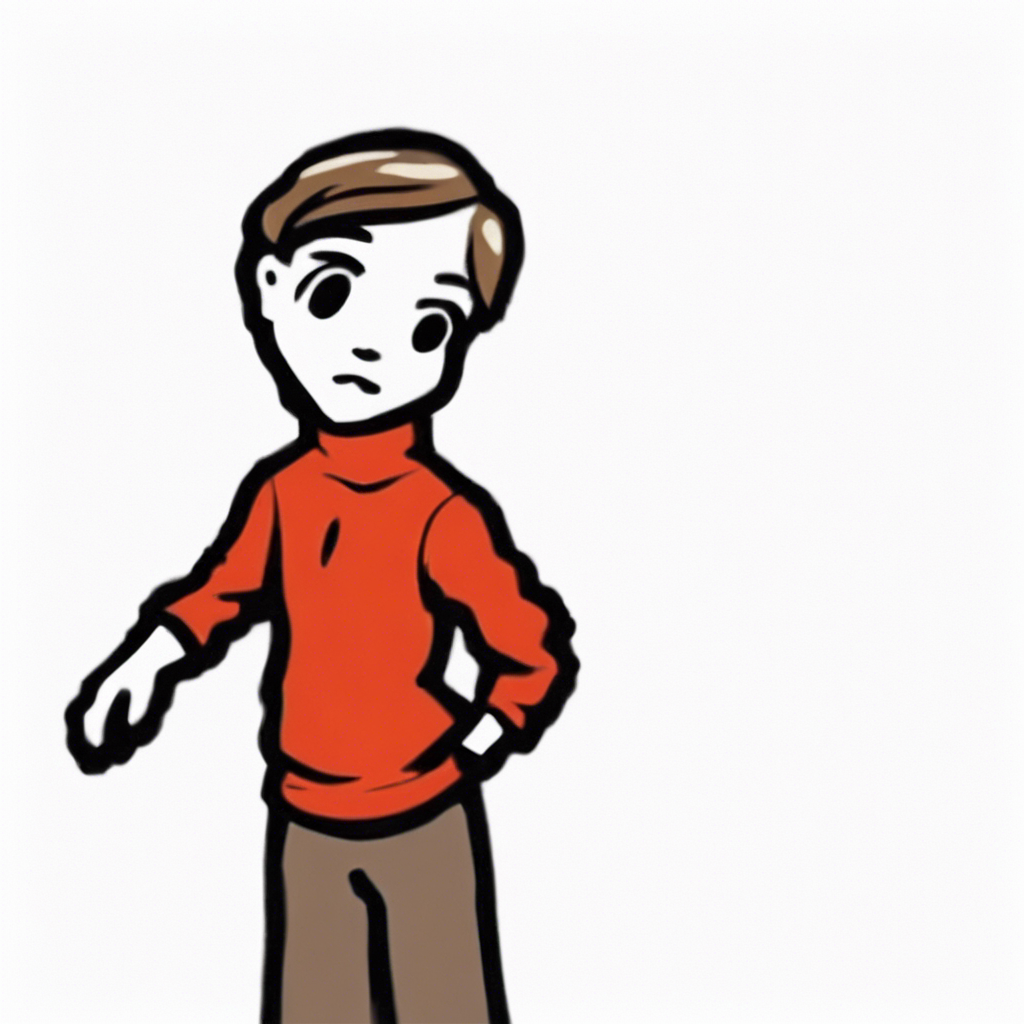
\includegraphics[width=0.5\linewidth]{img/Eva.png}
                    \\
                    \text{$Eva$}
                \end{figure}
                \begin{figure}
                    
\includegraphics[width=0.9\linewidth, height=0.15\textheight]{img/flecha_derecha.png}
                    \\
                    \text{$mensaje$}
                \end{figure}
            
                \column{0.33\textwidth}
                \centering
                \begin{figure}
                    \vspace{1.8cm}
                    
\includegraphics[width=0.5\linewidth]{img/Personaje_derecha.png}
                    \\
                    \text{Bob}
                \end{figure}
            \end{columns}
        \end{frame}

         \begin{frame}{Cifrado asimétrico}
            \begin{columns}
                \column{0.33\textwidth}
                \centering
                \begin{figure}
                    \vspace{1.8cm}
                    
\includegraphics[width=0.5\linewidth]{img/Personaje_izquierda.png}
                    \\
                    \text{Alice}
                \end{figure}
                \raggedright
                \begin{tikzpicture}
                    \hspace{0.8cm}
                    \node[draw, rectangle, minimum width=1cm, minimum height=0.7cm] at (0,0) {skA};
                    \hspace{1.5cm}
                    \node[draw, rectangle, minimum width=1cm, minimum height=0.7cm] at (0,0) {pkA};
                \end{tikzpicture}

                \column{0.33\textwidth}
                \centering
                \begin{figure}
                    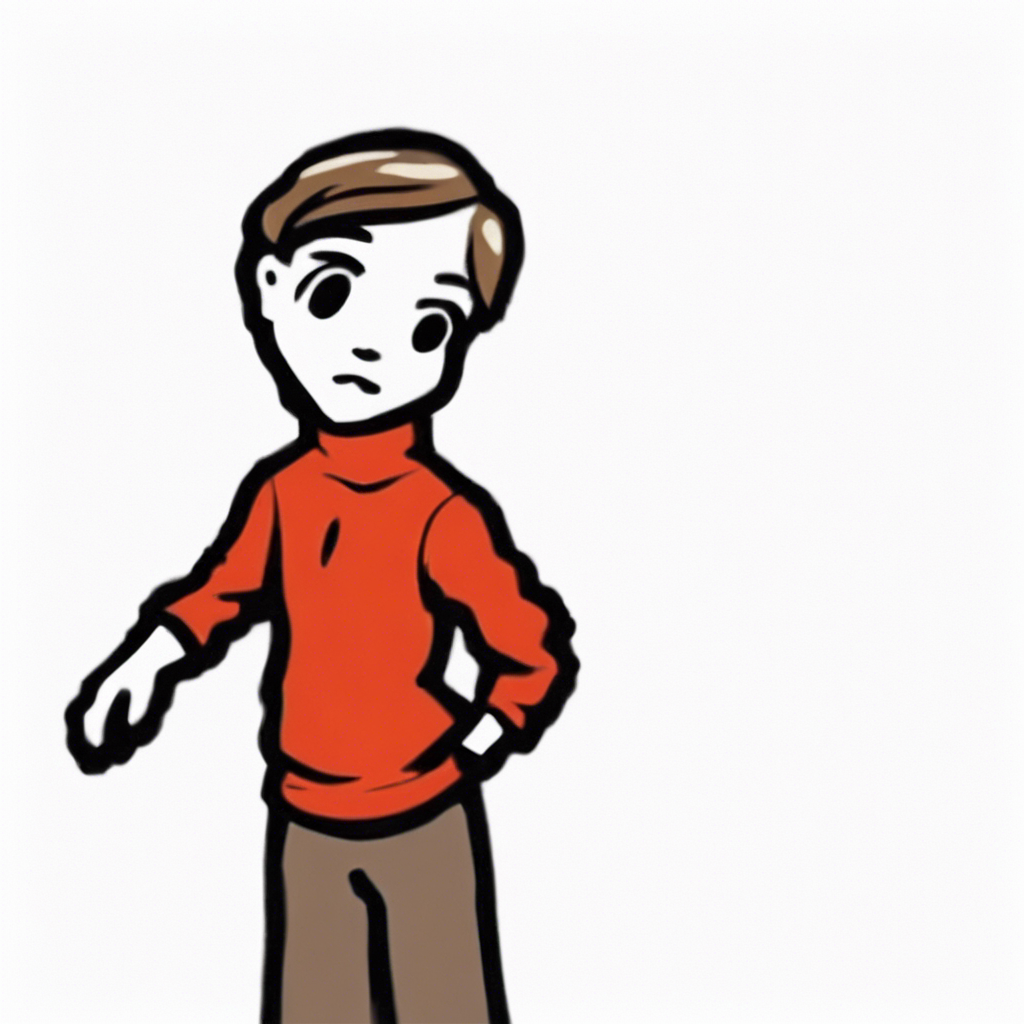
\includegraphics[width=0.5\linewidth]{img/Eva.png}
                    \\
                    \text{$Eva$}
                \end{figure}
                \begin{figure}
                    
\includegraphics[width=0.9\linewidth, height=0.15\textheight]{img/flecha_derecha.png}
                    \\
                    \text{$mensaje$}
                \end{figure}
            
                \column{0.33\textwidth}
                \centering
                \begin{figure}
                    \vspace{1.8cm}
                    
\includegraphics[width=0.5\linewidth]{img/Personaje_derecha.png}
                    \\
                    \text{Bob}
                \end{figure}
                \raggedright
                \begin{tikzpicture}
                    \hspace{0.8cm}
                    \node[draw, rectangle, minimum width=1cm, minimum height=0.7cm] at (0,0) {pkB};
                    \hspace{1.5cm}
                    \node[draw, rectangle, minimum width=1cm, minimum height=0.7cm] at (0,0) {skB};
                \end{tikzpicture}
            \end{columns}
        \end{frame}

        \begin{frame}{Cifrado asimétrico}
            \begin{columns}
                \column{0.33\textwidth}
                \centering
                \begin{figure}
                    \text{$enc_{pkB}(mensaje) = x$}
                    \\
                    \vspace{0.25cm}
                    
\includegraphics[width=0.2\linewidth, height=0.1\textheight]{img/flecha_misma.png}
                    \\
                    
\includegraphics[width=0.5\linewidth]{img/Personaje_izquierda.png}
                    \\
                    \text{Alice}
                \end{figure}
                \raggedright
                \begin{tikzpicture}
                    \hspace{0.8cm}
                    \node[draw, rectangle, minimum width=1cm, minimum height=0.7cm] at (0,0) {skA};
                    \hspace{1.5cm}
                    \node[draw, rectangle, minimum width=1cm, minimum height=0.7cm] at (0,0) {pkA};
                \end{tikzpicture}

                \column{0.33\textwidth}
                \centering
                \begin{figure}
                    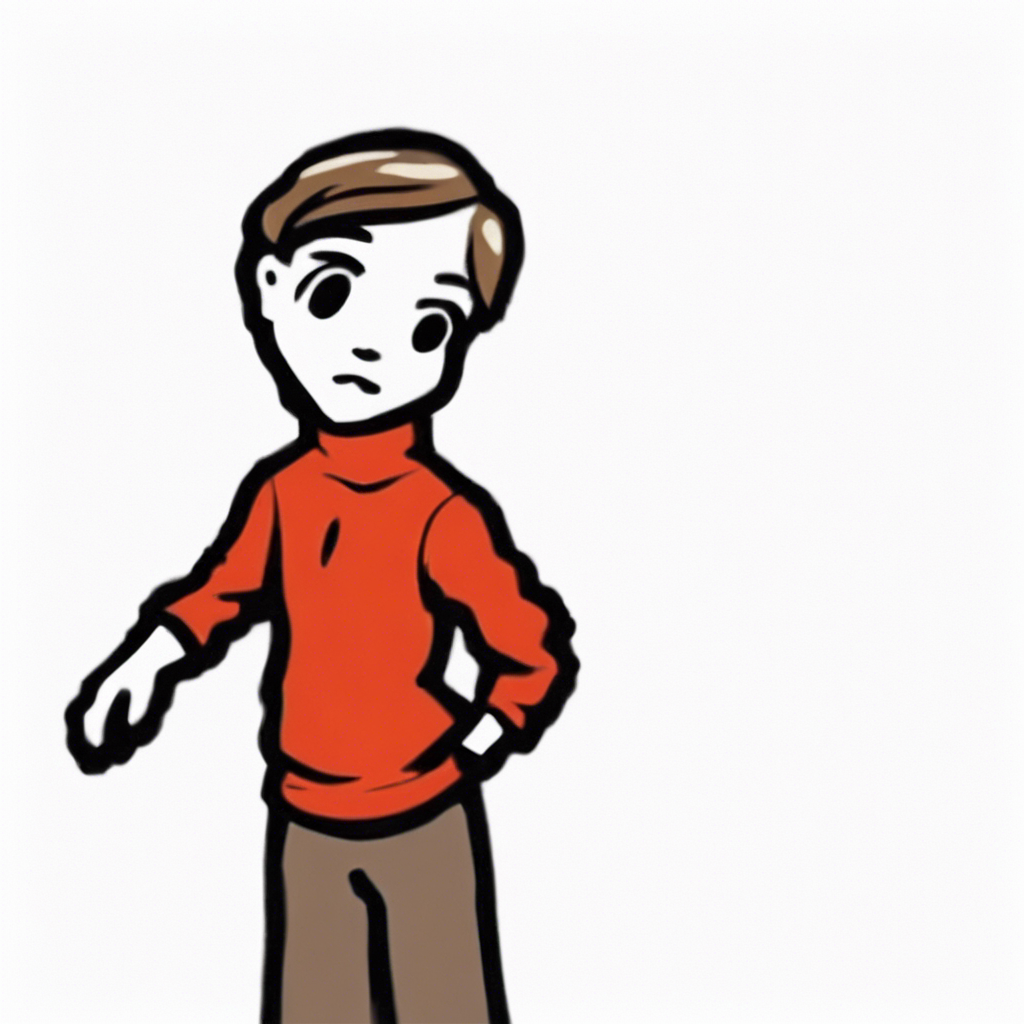
\includegraphics[width=0.5\linewidth]{img/Eva.png}
                    \\
                    \text{$Eva$}
                \end{figure}
                \begin{figure}
                    
\includegraphics[width=0.9\linewidth, height=0.15\textheight]{img/flecha_derecha.png}
                    \\
                    \text{$x$}
                \end{figure}
            
                \column{0.33\textwidth}
                \centering
                \begin{figure}
                    \vspace{1.8cm}
                    
\includegraphics[width=0.5\linewidth]{img/Personaje_derecha.png}
                    \\
                    \text{Bob}
                \end{figure}
                \raggedright
                \begin{tikzpicture}
                    \hspace{0.8cm}
                    \node[draw, rectangle, minimum width=1cm, minimum height=0.7cm] at (0,0) {pkB};
                    \hspace{1.5cm}
                    \node[draw, rectangle, minimum width=1cm, minimum height=0.7cm] at (0,0) {skB};
                \end{tikzpicture}
            \end{columns}
        \end{frame}

        \begin{frame}{Cifrado asimétrico}
            \begin{columns}
                \column{0.33\textwidth}
                \centering
                \begin{figure}
                    \text{$enc_{pkB}(mensaje) = x$}
                    \\
                    \vspace{0.25cm}
                    
\includegraphics[width=0.2\linewidth, height=0.1\textheight]{img/flecha_misma.png}
                    \\
                    
\includegraphics[width=0.5\linewidth]{img/Personaje_izquierda.png}
                    \\
                    \text{Alice}
                \end{figure}
                \raggedright
                \begin{tikzpicture}
                    \hspace{0.8cm}
                    \node[draw, rectangle, minimum width=1cm, minimum height=0.7cm] at (0,0) {skA};
                    \hspace{1.5cm}
                    \node[draw, rectangle, minimum width=1cm, minimum height=0.7cm] at (0,0) {pkA};
                \end{tikzpicture}

                \column{0.33\textwidth}
                \centering
                \begin{figure}
                    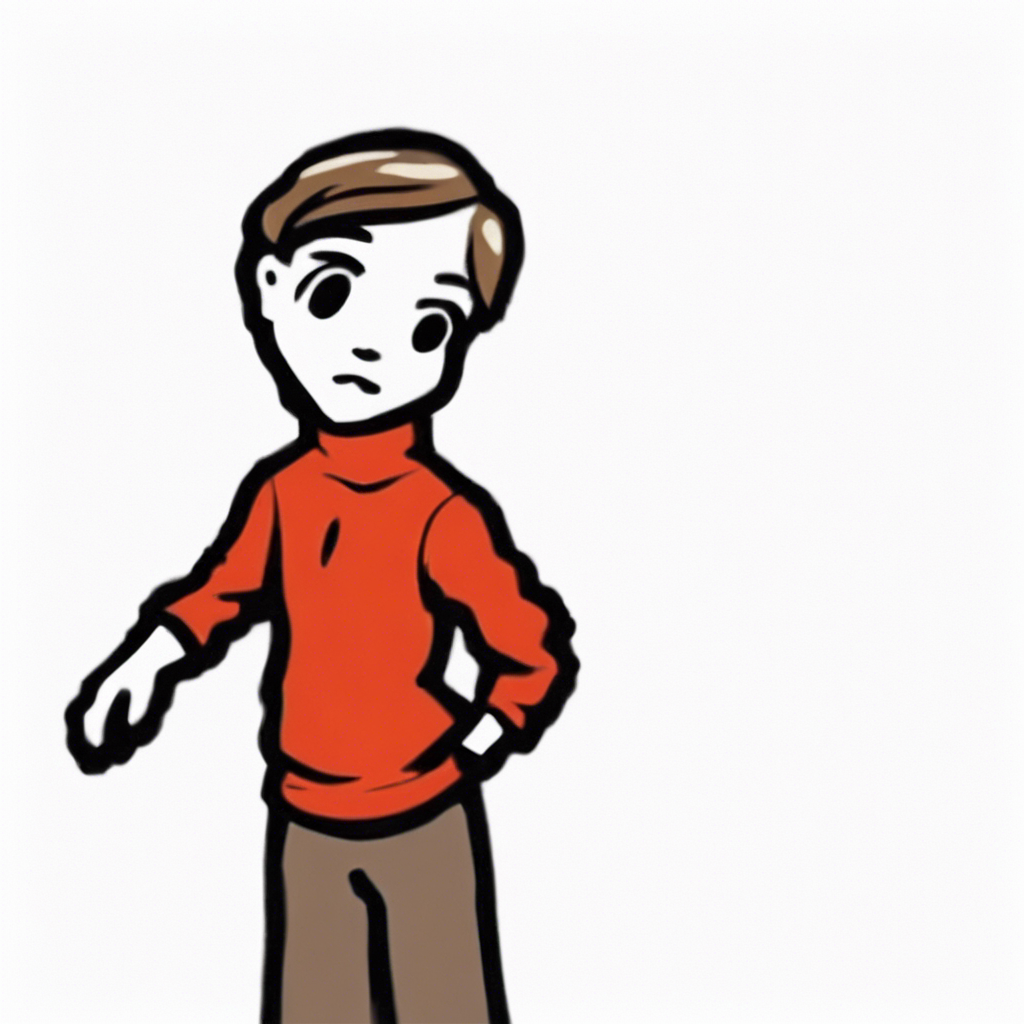
\includegraphics[width=0.5\linewidth]{img/Eva.png}
                    \\
                    \text{$Eva$}
                \end{figure}
                \begin{figure}
                    
\includegraphics[width=0.9\linewidth, height=0.15\textheight]{img/flecha_derecha.png}
                    \\
                    \text{$x$}
                \end{figure}
            
                \column{0.33\textwidth}
                \centering
                \begin{figure}
                    \text{$dec_{skB}(x) = mensaje$}
                    \\
                    \vspace{0.3cm}
                    
\includegraphics[width=0.2\linewidth, height=0.1\textheight]{img/flecha_misma.png}
                    \\
                    
\includegraphics[width=0.5\linewidth]{img/Personaje_derecha.png}
                    \\
                    \text{Bob}
                \end{figure}
                \raggedright
                \begin{tikzpicture}
                    \hspace{0.8cm}
                    \node[draw, rectangle, minimum width=1cm, minimum height=0.7cm] at (0,0) {pkB};
                    \hspace{1.5cm}
                    \node[draw, rectangle, minimum width=1cm, minimum height=0.7cm] at (0,0) {skB};
                \end{tikzpicture}
            \end{columns}
        \end{frame}

        \begin{frame}{Clasificación de los criptosistemas asimétricos}
            Algunas metodologías son:
            \begin{enumerate}
                \item Basados en el problema de la mochila
                \item Basados en retículos
                \item Basados en códigos
                \item Basados en curvas elípticas
                \item Basados en funciones hash
                \item Basados en ecuaciones cuadráticas multivariantes
            \end{enumerate}
            \vspace{2.4cm}
        \end{frame}

        \begin{frame}{Clasificación de los criptosistemas asimétricos}
            Algunas metodologías son:
            \begin{enumerate}
                \item Basados en el problema de la mochila
                \item Basados en retículos
                \item Basados en códigos
                \item Basados en curvas elípticas
                \item Basados en funciones hash
                \item Basados en ecuaciones cuadráticas multivariantes
            \end{enumerate}
            \vspace{0.6cm}
            Aunque, actualmente:
            \begin{enumerate}
                \item Criptosistemas resistentes a ataques cuánticos
                \item Criptosistemas no resistentes a estos ataques
            \end{enumerate}
        \end{frame}

    % Problema de la mochila
    \section{Problema de la mochila}

        \begin{frame}{Siete problemas del milenio}
            \begin{enumerate}
                \item La conjetura de Hodge
                \item La conjetura de Poincaré
                \item La hipótesis de Riemann
                \item Las ecuaciones de Navier-Stokes
                \item Existencia de Yang-Mills y del salto de masa
                \item La conjetura de Birch y Swinnerton-Dyer
                \item El problema P vs NP
            \end{enumerate}
        \end{frame}

        \begin{frame}{Siete problemas del milenio}
            \begin{enumerate}
                \item La conjetura de Hodge
                \item La conjetura de Poincaré
                \item La hipótesis de Riemann
                \item Las ecuaciones de Navier-Stokes
                \item Existencia de Yang-Mills y del salto de masa
                \item La conjetura de Birch y Swinnerton-Dyer
                \item \textbf{El problema P vs NP}
            \end{enumerate}
        \end{frame}

        \begin{frame}{Conjuntos P y NP}
            \begin{block}{Conjunto NP}
                Denominamos \textit{NP} al conjunto de problemas en los que podemos comprobar si una respuesta dada es correcta o no, en tiempo polinomial.
            \end{block}
            \begin{block}{Conjunto P}
                Denominamos \textit{P} al conjunto de problemas en los que podemos encontrar 
                una respuesta al problema, en tiempo polinomial.
            \end{block}
        \end{frame}

        \begin{frame}{P vs NP}
             \begin{columns}
                \column{0.5\textwidth}
                    \centering
                    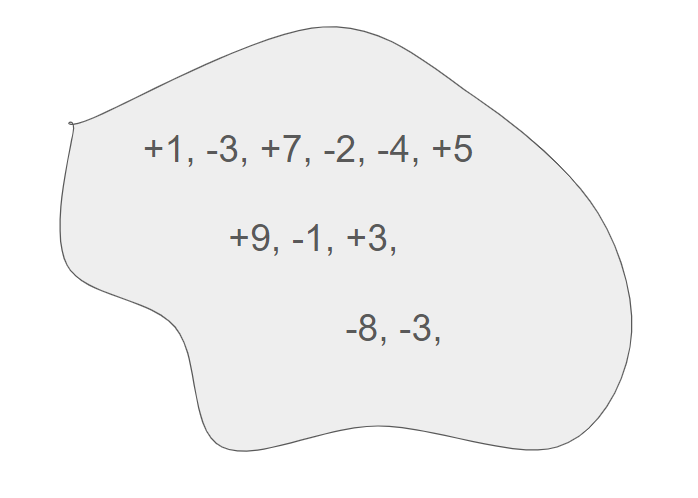
\includegraphics[width=\linewidth]{img/Nube_puntos.png}
                    \vspace{2cm}
                \column{0.5\textwidth}
                    \centering
                    Tomar varios de estos números \\ tal que su suma sea $0$                    \vspace{2.5cm}
            \end{columns}
        \end{frame}    

        \begin{frame}{P vs NP}
             \begin{columns}
                \column{0.5\textwidth}
                    \centering
                    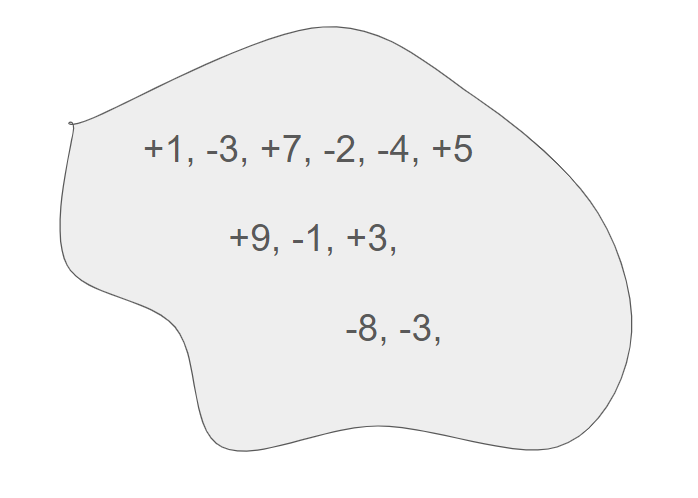
\includegraphics[width=\linewidth]{img/Nube_puntos.png}
                    \vspace{2cm}
                    
                \column{0.5\textwidth}
                    \centering
                    $\{-3, +7, -4\}$
                    \\ \vspace{0.25cm}
                    $\Downarrow$ 
                    \\ \vspace{0.25cm}
                    $-3 + 7 - 4 = 0$
                    \\ \vspace{2.5cm}
            \end{columns}
        \end{frame}    

        \begin{frame}{P vs NP}
             \begin{columns}
                \column{0.5\textwidth}
                    \centering
                    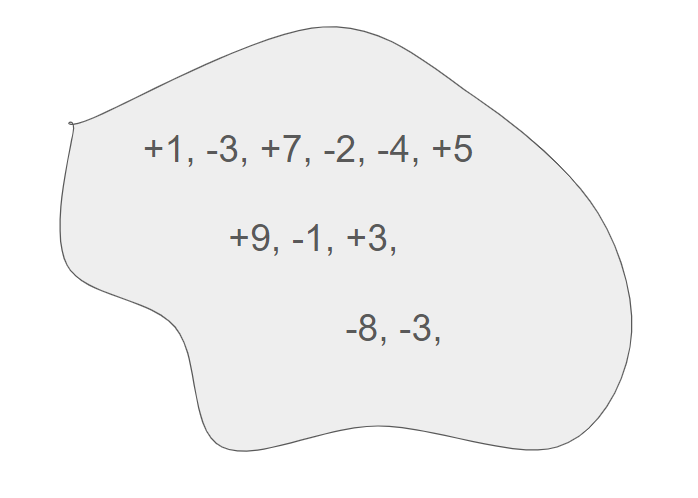
\includegraphics[width=\linewidth]{img/Nube_puntos.png}
                    
                \column{0.5\textwidth}
                    \centering
                    $\{-3, +7, -4\}$
                    \\ \vspace{0.25cm}
                    $\Downarrow$ 
                    \\ \vspace{0.25cm}
                    $-3 + 7 - 4 = 0$
            \end{columns}
            \vspace{0.5cm}
            Es claro que $P \subset NP$, pero ¿$NP \subset P$?
            \begin{block}{Problema P vs NP}
                ¿P = NP?
            \end{block}
        \end{frame}     

        \begin{frame}{Problemas NP-Completos (I)}
            \begin{block}{Reducción}
                Llamamos \textit{reducción} a una transformación en tiempo polinomial, de un problema de decisión en otro equivalente. Esto es, sea $A$ el conjunto de instancias del primer problema, y $B$ el conjunto de instancias del segundo, definimos una reducción $r$ como $r : A \rightarrow B$ tal que: 
                \begin{equation*}
                    a \in A \text{ es sí } \iff r(a) \in B \text{ es sí }
                \end{equation*}
            \end{block}
            \begin{block}{Problema NP-Completo}
                Diremos que un problema es \textit{NP-completo} si es un problema de decisión perteneciente a $NP$, que además verifica que existe una reducción de cada problema de $NP$ a él.
            \end{block}
        \end{frame}
    
        \begin{frame}{Problemas NP-Completos (II)}
            \centering
            \includegraphics[width=0.8\linewidth, height=0.8\textheight]{img/NP-Completo.png}
        \end{frame}

        \begin{frame}{Problema de la mochila (I)}
            \begin{columns}
                \column{0.4\textwidth}
                \centering
                \vspace{1cm}
                \begin{figure}
                    \includegraphics[width=0.9\linewidth, height=0.3\textheight]{img/Gafas_sol.png}
                \end{figure}
                Tamaño = 7 \\
                Peso = 2

                \column{0.2\textwidth}
                
                \column{0.4\textwidth}
                \centering
                \vspace{1cm}
                \begin{figure}
                    \includegraphics[width=\linewidth, height=0.3\textheight]{img/Tijeras.png}
                \end{figure}
                Tamaño = 6 \\
                Peso = 4
            \end{columns}
        \end{frame}

        \begin{frame}{Problema de la mochila (I)}
            \begin{columns}
                \column{0.4\textwidth}
                \centering
                \vspace{1cm}
                \begin{figure}
                    \includegraphics[width=0.9\linewidth, height=0.3\textheight]{img/Gafas_sol.png}
                \end{figure}
                Tamaño = 7 \\
                Peso = 2

                \column{0.2\textwidth}
                \vspace{-2cm}
                \begin{figure}
                    \hspace*{-2.6cm}
                    \includegraphics[width=8cm, height=0.6\textheight]{img/Mochila.png}
                \end{figure}
                
                \column{0.4\textwidth}
                \centering
                \vspace{1cm}
                \begin{figure}
                    \includegraphics[width=\linewidth, height=0.3\textheight]{img/Tijeras.png}
                \end{figure}
                Tamaño = 6 \\
                Peso = 4
            \end{columns}
        \end{frame}

        \begin{frame}{Problema de la mochila (II)}
            \begin{block}{Definición}
                Sean $a = \{ a_{1}, ... , a_{n}\} \subseteq \mathbb{N}^{*}$ un \textit{conjunto de pesos} y S $\in \mathbb{N}^{*}$ la \textit{capacidad total}, el \textit{problema de la mochila} busca encontrar el \textit{vector de soluciones} $x = \{ x_{1}, ... , x_{n} \} \subseteq \mathbb{N}^{*}$ que maximice el valor de la mochila y verifique:
                \begin{equation*} 
                    \sum_{i=1}^{n} a_{i} \cdot x_{i} \leq S 
                \end{equation*}
            \end{block}
            \vspace{0.5cm}
            En particular, nosotros nos centraremos en:
            \begin{equation*} 
                \sum_{i=1}^{n} a_{i} \cdot x_{i} = S 
            \end{equation*}
        \end{frame}

    % Criptosistema de Merkle-Hellman
    \section{Criptosistema de Merkle-Hellman}
    \subsection{Método básico}

        \begin{frame}{Sucesión supercreciente}
            \begin{block}{Definición}
                Diremos que una sucesión $\{a_i\}_{i=1}^{n}$ es \textit{supercreciente} si verifica que:
                \begin{equation*}
                    a_{i} > \sum_{j=1}^{i-1} a_{j} \text{ , para } i = 2, ... , n
                \end{equation*}
            \end{block}
            Por ejemplo, $\{a_{n}\} = 1, 3, 8, 16, ...$ es supercreciente ya que:
            \begin{align*}
                a_{2} = 3  &> a_{1} = 1 \\ 
                a_{3} = 8  &> \sum_{i=1}^{2} a_{i} = 3 + 1 = 4 \\
                a_{4} = 16 &> \sum_{i=1}^{3} a_{i} = 4 + 8 = 12 
            \end{align*}
        \end{frame}
    
        \begin{frame}{Idea del método básico}
            \centering
            $S' = a' \cdot mensaje$
            \\ \vspace{0.25cm}
            $\Downarrow$
            \\ \vspace{0.25cm}
            $S = a \cdot mensaje$
        \end{frame}

        \begin{frame}{Idea del método básico}
            \centering
            $S' = a' \cdot mensaje$
            \\ \vspace{0.25cm}
            $\Uparrow$
            \\ \vspace{0.25cm}
            $S = a \cdot mensaje$
        \end{frame}

        \begin{frame}{Método básico}
            \begin{columns}
                \column{0.33\textwidth}
                \centering
                \begin{figure}
                    \vspace{1.75cm}
                    \includegraphics[width=0.5\linewidth]{img/Personaje_izquierda.png}
                    \\
                    \text{Alice}
                \end{figure}

                \column{0.33\textwidth}
                \centering
                \begin{figure}
                    \includegraphics[width=0.5\linewidth]{img/Eva.png}
                    \\
                    \text{$Eva$}
                \end{figure}
                \begin{figure}
                    \includegraphics[width=0.9\linewidth, height=0.15\textheight]{img/flecha_izquierda.png}
                \end{figure}
            
                \column{0.33\textwidth}
                \centering
                \begin{figure}
                    \vspace{1.8cm}
                    \includegraphics[width=0.5\linewidth]{img/Personaje_derecha.png}
                    \\
                    \text{Bob}
                \end{figure}
            \end{columns}
        \end{frame}

        \begin{frame}{Método básico}
            \begin{columns}
                \column{0.33\textwidth}
                \centering
                \begin{figure}
                    \text{Generación claves}
                    \\
                    \vspace{0.25cm}
                    \includegraphics[width=0.2\linewidth, height=0.1\textheight]{img/flecha_misma.png}
                    \\
                    \includegraphics[width=0.5\linewidth]{img/Personaje_izquierda.png}
                    \\
                    \text{Alice}
                \end{figure}

                \column{0.33\textwidth}
                \centering
                \begin{figure}
                    \includegraphics[width=0.5\linewidth]{img/Eva.png}
                    \\
                    \text{$Eva$}
                \end{figure}
                \vspace{1.7cm}
            
                \column{0.33\textwidth}
                \centering
                \begin{figure}
                    \vspace{1.8cm}
                    \includegraphics[width=0.5\linewidth]{img/Personaje_derecha.png}
                    \\
                    \text{Bob}
                \end{figure}
            \end{columns}
        \end{frame}

        \begin{frame}{Generación de claves}
            \begin{itemize}
                \item Generación de clave privada
                \\ \vspace{1.5cm}
                \item Generación de clave pública
                \vspace{2cm}
            \end{itemize}
        \end{frame}

        \begin{frame}{Generación de claves}
            \begin{itemize}
                \item \textbf{Generación de clave privada}
                \begin{itemize}[label=--]
                    \item Valores coprimos $m$ y $w$, esto es, $mcd(m, w) = 1$ 
                    \item Sucesión supercreciente $a'$ 
                \end{itemize}
                \begin{equation*}
                    sk = (m, w, a')    
                \end{equation*}
                \item Generación de clave pública
                \vspace{2cm}
            \end{itemize}
        \end{frame}

        \begin{frame}{Generación de claves}
            \begin{itemize}
                \item Generación de clave privada
                \begin{itemize}[label=--]
                    \item Valores coprimos $m$ y $w$, esto es, $mcd(m, w) = 1$ 
                    \item Sucesión supercreciente $a'$ 
                \end{itemize}
                \begin{equation*}
                    sk = (m, w, a')    
                \end{equation*}
                \item \textbf{Generación de clave pública}
                \begin{align*}
                    a_{i} &\equiv w \cdot a'_{i} \text{ (mod } m) \text{, con } i = 1, ... , n \\
                    pk &= a
                \end{align*}
            \end{itemize}
        \end{frame}

        \begin{frame}{Método básico}
            \begin{columns}
                \column{0.33\textwidth}
                \centering
                \begin{figure}
                    \vspace{1.75cm}
                    \includegraphics[width=0.5\linewidth]{img/Personaje_izquierda.png}
                    \\
                    \text{Alice}
                \end{figure}
                \raggedright
                \begin{tikzpicture}
                    \hspace{0.8cm}
                    \node[draw, rectangle, minimum width=1cm, minimum height=0.7cm] at (0,0) {sk};
                    \hspace{1.5cm}
                    \node[draw, rectangle, minimum width=1cm, minimum height=0.7cm] at (0,0) {pk};
                \end{tikzpicture}

                \column{0.33\textwidth}
                \centering
                \begin{figure}
                    \includegraphics[width=0.5\linewidth]{img/Eva.png}
                    \\
                    \text{$Eva$}
                \end{figure}
                \begin{figure}
                    \includegraphics[width=0.9\linewidth, height=0.15\textheight]{img/flecha_izquierda.png}
                \end{figure}
            
                \column{0.33\textwidth}
                \centering
                \begin{figure}
                    \vspace{1.8cm}
                    \includegraphics[width=0.5\linewidth]{img/Personaje_derecha.png}
                    \\
                    \text{Bob}
                \end{figure}
            \end{columns}
        \end{frame}

        \begin{frame}{Método básico}
            \begin{columns}
                \column{0.33\textwidth}
                \centering
                \begin{figure}
                    \vspace{1.75cm}
                    \includegraphics[width=0.5\linewidth]{img/Personaje_izquierda.png}
                    \\
                    \text{Alice}
                \end{figure}
                \raggedright
                \begin{tikzpicture}
                    \hspace{0.8cm}
                    \node[draw, rectangle, minimum width=1cm, minimum height=0.7cm] at (0,0) {sk};
                    \hspace{1.5cm}
                    \node[draw, rectangle, minimum width=1cm, minimum height=0.7cm] at (0,0) {pk};
                \end{tikzpicture}

                \column{0.33\textwidth}
                \centering
                \begin{figure}
                    \includegraphics[width=0.5\linewidth]{img/Eva.png}
                    \\
                    \text{$Eva$}
                \end{figure}
                \begin{figure}
                    \includegraphics[width=0.9\linewidth, height=0.15\textheight]{img/flecha_izquierda.png}
                \end{figure}
            
                \column{0.33\textwidth}
                \centering
                \begin{figure}
                    \text{Cifrado}
                    \\
                    \vspace{0.25cm}
                    \includegraphics[width=0.2\linewidth, height=0.1\textheight]{img/flecha_misma.png}
                    \\
                    \includegraphics[width=0.5\linewidth]{img/Personaje_derecha.png}
                    \\
                    \text{Bob}
                \end{figure}
            \end{columns}
        \end{frame}

        \begin{frame}{Cifrado}
            Se necesita:
            \\ \vspace{0.25cm}
            \begin{itemize}
                \item Clave pública $pk = (a_{1}, ... , a_{n})$
                \vspace{0.25cm}
                \item Mensaje $m = (m_{1}, ... , m_{n})$
            \end{itemize}
            \vspace{1cm}
            Cálculo del mensaje cifrado:
            \begin{equation*}
                S = pk \cdot m = \sum_{i=1}^{n} a_{i} \cdot m_{i}
            \end{equation*}
        \end{frame}

        \begin{frame}{Método básico}
            \begin{columns}
                \column{0.33\textwidth}
                \centering
                \begin{figure}
                    \vspace{1.75cm}
                    \includegraphics[width=0.5\linewidth]{img/Personaje_izquierda.png}
                    \\
                    \text{Alice}
                \end{figure}
                \raggedright
                \begin{tikzpicture}
                    \hspace{0.8cm}
                    \node[draw, rectangle, minimum width=1cm, minimum height=0.7cm] at (0,0) {sk};
                    \hspace{1.5cm}
                    \node[draw, rectangle, minimum width=1cm, minimum height=0.7cm] at (0,0) {pk};
                \end{tikzpicture}

                \column{0.33\textwidth}
                \centering
                \begin{figure}
                    \includegraphics[width=0.5\linewidth]{img/Eva.png}
                    \\
                    \text{$Eva$}
                \end{figure}
                \begin{figure}
                    \includegraphics[width=0.9\linewidth, height=0.15\textheight]{img/flecha_izquierda.png}
                    \\ \vspace{0.5cm}
                \end{figure}
            
                \column{0.33\textwidth}
                \centering
                \begin{figure}
                    \vspace{1.8cm}
                    \includegraphics[width=0.5\linewidth]{img/Personaje_derecha.png}
                    \\
                    \text{Bob}
                \end{figure}
            \end{columns}
        \end{frame}

        \begin{frame}{Método básico}
            \begin{columns}
                \column{0.33\textwidth}
                \centering
                \begin{figure}
                    \vspace{1.75cm}
                    \includegraphics[width=0.5\linewidth]{img/Personaje_izquierda.png}
                    \\
                    \text{Alice}
                \end{figure}
                \raggedright
                \begin{tikzpicture}
                    \hspace{0.8cm}
                    \node[draw, rectangle, minimum width=1cm, minimum height=0.7cm] at (0,0) {sk};
                    \hspace{1.5cm}
                    \node[draw, rectangle, minimum width=1cm, minimum height=0.7cm] at (0,0) {pk};
                \end{tikzpicture}

                \column{0.33\textwidth}
                \centering
                \begin{figure}
                    \includegraphics[width=0.5\linewidth]{img/Eva.png}
                    \\
                    \text{$Eva$}
                \end{figure}
                \begin{figure}
                    \includegraphics[width=0.9\linewidth, height=0.15\textheight]{img/flecha_izquierda.png}
                    \\
                    \text{$S$}
                \end{figure}
            
                \column{0.33\textwidth}
                \centering
                \begin{figure}
                    \vspace{1.8cm}
                    \includegraphics[width=0.5\linewidth]{img/Personaje_derecha.png}
                    \\
                    \text{Bob}
                \end{figure}
            \end{columns}
        \end{frame}

        \begin{frame}{Método básico}
            \begin{columns}
                \column{0.33\textwidth}
                \centering
                \begin{figure}
                    \text{Descifrado}
                    \\
                    \vspace{0.25cm}
                    \includegraphics[width=0.2\linewidth, height=0.1\textheight]{img/flecha_misma.png}
                    \\
                    \includegraphics[width=0.5\linewidth]{img/Personaje_izquierda.png}
                    \\
                    \text{Alice}
                \end{figure}
                \raggedright
                \begin{tikzpicture}
                    \hspace{0.8cm}
                    \node[draw, rectangle, minimum width=1cm, minimum height=0.7cm] at (0,0) {sk};
                    \hspace{1.5cm}
                    \node[draw, rectangle, minimum width=1cm, minimum height=0.7cm] at (0,0) {pk};
                \end{tikzpicture}

                \column{0.33\textwidth}
                \centering
                \begin{figure}
                    \includegraphics[width=0.5\linewidth]{img/Eva.png}
                    \\
                    \text{$Eva$}
                \end{figure}
                \begin{figure}
                    \includegraphics[width=0.9\linewidth, height=0.15\textheight]{img/flecha_izquierda.png}
                    \\
                    \text{$S$}
                \end{figure}
            
                \column{0.33\textwidth}
                \centering
                \begin{figure}
                    \vspace{1.8cm}
                    \includegraphics[width=0.5\linewidth]{img/Personaje_derecha.png}
                    \\
                    \text{Bob}
                \end{figure}
            \end{columns}
        \end{frame}

        \begin{frame}{Descifrado (I)}
            Se necesita:
            \\ \vspace{0.25cm}
            \begin{itemize}
                \item Clave privada $sk = (m, w, a')$
                \vspace{0.25cm}
                \item Mensaje cifrado $S$
            \end{itemize}
            \vspace{1cm}
            Cálculo del mensaje descifrado:
            \begin{equation*}
                S' = w^{-1} \cdot S \text{ (mod } m)
            \end{equation*}
        \end{frame}

        \begin{frame}{Descifrado (II)}
            Conseguir el mensaje $x = (x_{1}, ... , x_{n})$ descifrado a partir de $S'$:
            \vspace{0.25cm}
            \begin{align*}
                x_{n} = 1 &\iff S' \geq a'_{n} \\
                x_{i} = 1 &\iff S' \geq a'_{i} + \sum_{j=i+1}^{n} a'_{j} \cdot x_{j} 
            \end{align*}
            con $i = n-1, ... , 1$.
        \end{frame}

        \begin{frame}{Ejemplo de descifrado}
            \begin{center}
                \textbf{\uline{Ejemplo}}
            \end{center}
            \vspace{0.25cm}
            Para el mensaje = $(0, 0, 0, 1, 1)$, generamos:
            \\ \vspace{0.25cm}
            $S' = 744$, $n = 5$, y $a' = (3, 42, 105, 249, 495)$
            \begin{align*}
                S' = 744 &\geq a'_{5} = 495 \Rightarrow x_{5} = 1 \\
                S' = 744 &\geq a'_{5} + a'_{4} = 744 \Rightarrow x_{4} = 1 \\
                S' = 744 &\not\geq a'_{5} + a'_{4} + a'_{3} = 849 \Rightarrow x_{3} = 0 \\
                &\hspace{0.2cm}\vdots
            \end{align*}
            Finalmente, obtenemos $x = (0, 0, 0, 1, 1)$.
        \end{frame}

    \subsection{Método iterativo}

        \begin{frame}{Idea del método iterativo}
            \begin{columns}
                \column{0.5\textwidth}
                Datos generados
                \begin{itemize}
                    \item Valores coprimos: $m, w$
                    \item Sucesión supercreciente: $a'$
                \end{itemize}
                \vspace{0.5cm}
                Datos recibidos
                \begin{itemize}
                    \item Mensaje cifrado: $S$
                \end{itemize}
                \vspace{0.5cm}
                Datos objetivo
                \begin{itemize}
                    \item Clave pública: $a$
                    \item Mensaje transformado: $S'$
                \end{itemize}

                \column{0.5\textwidth}
                \centering
                $S' = a' \cdot mensaje$
                \\ \vspace{0.25cm}
                $\Downarrow$
                \\ \vspace{0.25cm}
                $S = a \cdot mensaje$
            \end{columns}
        \end{frame}

        \begin{frame}{Idea del método iterativo}
            \begin{columns}
                \column{0.5\textwidth}
                Datos generados
                \begin{itemize}
                    \item Valores coprimos: $m, w$
                    \item Sucesión supercreciente: $a'$
                \end{itemize}
                \vspace{0.5cm}
                Datos recibidos
                \begin{itemize}
                    \item Mensaje cifrado: $S$
                \end{itemize}
                \vspace{0.5cm}
                Datos objetivo
                \begin{itemize}
                    \item Clave pública: $a$
                    \item Mensaje transformado: $S'$
                \end{itemize}

                \column{0.5\textwidth}
                \centering
                $S'' = a'' \cdot mensaje$
                \\ \vspace{0.25cm}
                $\Downarrow$
                \\ \vspace{0.25cm}
                $S' = a' \cdot mensaje$
                \\ \vspace{0.25cm}
                $\Downarrow$
                \\ \vspace{0.25cm}
                $S = a \cdot mensaje$
            \end{columns}
        \end{frame}

        \begin{frame}{Idea del método iterativo}
            \begin{columns}
                \column{0.5\textwidth}
                Datos generados
                \begin{itemize}
                    \item Valores coprimos: $m, w$
                    \item Sucesión supercreciente: $a'$
                \end{itemize}
                \vspace{0.5cm}
                Datos recibidos
                \begin{itemize}
                    \item Mensaje cifrado: $S$
                \end{itemize}
                \vspace{0.5cm}
                Datos objetivo
                \begin{itemize}
                    \item Clave pública: $a$
                    \item Mensaje transformado: $S'$
                \end{itemize}

                \column{0.5\textwidth}
                \centering
                $S''' = a''' \cdot mensaje$
                \\ \vspace{0.25cm}
                $\Downarrow$
                \\ \vspace{0.25cm}
                $S'' = a'' \cdot mensaje$
                \\ \vspace{0.25cm}
                $\Downarrow$
                \\ \vspace{0.25cm}
                $S' = a' \cdot mensaje$
                \\ \vspace{0.25cm}
                $\Downarrow$
                \\ \vspace{0.25cm}
                $S = a \cdot mensaje$
            \end{columns}
        \end{frame}

        \begin{frame}{Idea del método iterativo}
            \begin{columns}
                \column{0.5\textwidth}
                Datos generados
                \begin{itemize}
                    \item Valores coprimos: $m, w$
                    \item Sucesión supercreciente: $a'$
                \end{itemize}
                \vspace{0.5cm}
                Datos recibidos
                \begin{itemize}
                    \item Mensaje cifrado: $S$
                \end{itemize}
                \vspace{0.5cm}
                Datos objetivo
                \begin{itemize}
                    \item Clave pública: $a$
                    \item Mensaje transformado: $S'$
                \end{itemize}

                \column{0.5\textwidth}
                \centering
                ...
                \\ \vspace{0.25cm}
                $\Downarrow$ 
                \\ \vspace{0.25cm}
                $S''' = a''' \cdot mensaje$
                \\ \vspace{0.25cm}
                $\Downarrow$
                \\ \vspace{0.25cm}
                $S'' = a'' \cdot mensaje$
                \\ \vspace{0.25cm}
                $\Downarrow$
                \\ \vspace{0.25cm}
                $S' = a' \cdot mensaje$
                \\ \vspace{0.25cm}
                $\Downarrow$
                \\ \vspace{0.25cm}
                $S = a \cdot mensaje$
            \end{columns}
        \end{frame}

        \begin{frame}{Método iterativo}
            \begin{columns}
                \column{0.5\textwidth}
                \centering
                \textbf{\uline{Método Iterativo}}
                \\ \vspace{0.5cm}
                Cálculo de la clave pública:
                \begin{equation*}
                    a = w^{-1} \cdot a^{'} \text{ (mod } m)
                \end{equation*}
                Cálculo del mensaje transformado: 
                \begin{equation*}
                    S^{'} = w \cdot S \text{ (mod } m)
                \end{equation*}

                \column{0.5\textwidth}
                \centering
                \textbf{\uline{Método Básico}}
                \\ \vspace{0.5cm}
                Cálculo de la clave pública:
                \begin{equation*}
                    a = w \cdot a^{'} \text{ (mod } m)
                \end{equation*}
                Cálculo del mensaje transformado: 
                \begin{equation*}
                    S^{'} = w^{-1} \cdot S \text{ (mod } m)
                \end{equation*}
            \end{columns}
        \end{frame}

    % Ataques a este criptosistema
    \section{Ataques a este criptosistema}
    \subsection{Shamir}

        \begin{frame}{Ataques a Merkle-Hellman}
            \centering
            \begin{itemize}
                \item Ataque de Shamir
                \item Ataques por baja densidad
            \end{itemize}
        \end{frame}

        \begin{frame}{Ataques a Merkle-Hellman}
            \centering
            \begin{itemize}
                \item \textbf{Ataque de Shamir}
                \item Ataques por baja densidad
            \end{itemize}
        \end{frame}

        \begin{frame}{Idea de Shamir}             
            \centering
            \textbf{\uline{Objetivo Shamir}}
            \vspace{0.5cm}
            \begin{enumerate}
                \item Encontrar $m$ y $w$ para generar $a'$
                \begin{equation*}
                    a'_{i} \equiv w \cdot a_{i} \text{ mod } m
                \end{equation*}
                \item Obtener $S'$ usando $m$, $w$ y $S$:
                \begin{equation*}
                    S' = w^{-1} \cdot S \text{ (mod } m )
                \end{equation*}
                \item Usar $S'$ y $a'$ para obtener el mensaje
            \end{enumerate}
        \end{frame}

        \begin{frame}{Shamir}
            \begin{columns}
                \column{0.6\textwidth}
                \begin{figure}
                    \includegraphics[width=0.8\linewidth, height=0.5\textheight]{img/Grafica_Shamir.png}
                    \caption{Gráfica de la función $W \cdot a_{i} \text{ (mod } M_{0})$}
                \end{figure}

                \column{0.4\textwidth}
                \begin{itemize}
                    \item Eje horizontal: $W$
                    \item Eje vertical: $M_{0}$
                    \item Pendiente: $a_{i}$
                \end{itemize}
            \end{columns}
        \end{frame}

        \begin{frame}{Shamir}
            \begin{columns}
                \column{0.6\textwidth}
                \begin{figure}
                    \includegraphics[width=0.8\linewidth, height=0.5\textheight]{img/Grafica_Shamir.png}
                    \caption{Gráfica de la función $W \cdot a_{i} \text{ (mod } M_{0})$}
                \end{figure}

                \column{0.4\textwidth}
                \centering
                $a'_{1} = W_{0} \cdot a_{1} \text{ (mod } M_{0})$
                \\ \vspace{0.25cm}
                $\Downarrow$
                \\ \vspace{0.25cm}
                $d(W_{0}, minimo \text{ } a_{1}) \approx 2^{-n+1}$
            \end{columns}
        \end{frame}

        \begin{frame}{Shamir}
            \begin{columns}
                \column{0.6\textwidth}
                \begin{figure}
                    \includegraphics[width=0.8\linewidth, height=0.5\textheight]{img/Grafica_Shamir.png}
                    \caption{Gráfica de la función $W \cdot a_{i} \text{ (mod } M_{0})$}
                \end{figure}

                \column{0.4\textwidth}
                \centering
                $a'_{2} = W_{0} \cdot a_{2} \text{ (mod } M_{0})$
                \\ \vspace{0.25cm}
                $\Downarrow$
                \\ \vspace{0.25cm}
                $d(W_{0}, minimo \text{ } a_{2}) \approx 2^{-n+1}$
            \end{columns}
        \end{frame}

        \begin{frame}{Shamir}
            \begin{columns}
                \column{0.6\textwidth}
                \begin{figure}
                    \includegraphics[width=0.8\linewidth, height=0.5\textheight]{img/Grafica_Shamir.png}
                    \caption{Gráfica de la función $W \cdot a_{i} \text{ (mod } M_{0})$}
                \end{figure}

                \column{0.4\textwidth}
                \centering
                \textbf{...}
            \end{columns}
        \end{frame}

        \begin{frame}{Shamir}
            \begin{columns}
                \column{0.6\textwidth}
                \begin{figure}
                    \includegraphics[width=0.8\linewidth, height=0.5\textheight]{img/Grafica_Shamir.png}
                    \caption{Gráfica de la función $W \cdot a_{i} \text{ (mod } M_{0})$}
                \end{figure}

                \column{0.4\textwidth}
                \centering
                Puntos de acumulación
            \end{columns}
        \end{frame}

        \begin{frame}{Shamir}
            \begin{columns}
                \column{0.4\textwidth}
                \centering
                Dividir por $M_{0}$
                \\ \vspace{1cm}
                \begin{itemize}
                    \item $l$: nº curvas superpuestas
                    \item $k$: nº puntos acumulación
                \end{itemize}
                    
                \column{0.6\textwidth}
                \begin{figure}
                    \centering
                    \includegraphics[width=0.8\linewidth, height=0.5\textheight]{img/Grafica_Shamir_Dividida.png}
                    \caption{Gráfica de la función $V \cdot a_{i} \text{ (mod } 1)$}
                \end{figure}
            \end{columns}
        \end{frame}

        \begin{frame}{Shamir}
            \centering
            \begin{align*}
                \text{Sean } p,q,r, ... , \text{ enteros, } &&1 \leq p \leq a_{1} - 1 \\
                -\epsilon_{2} \leq \frac{p}{a_{1}}-\frac{q}{a_{2}} \leq \epsilon'_{2} &&1 \leq q \leq a_{2} - 1 \\
                -\epsilon_{3} \leq \frac{p}{a_{1}}-\frac{r}{a_{3}} \leq \epsilon'_{3} &&1 \leq r \leq a_{3} - 1
            \end{align*}
            $\Downarrow$
            \begin{align*}
                -\delta_{2} \leq pa_{2} &- qa_{1} \leq \delta'_{2} \\
                -\delta_{3} \leq pa_{3} &- ra_{1} \leq \delta'_{3} \\
                &\vdots
            \end{align*}
        \end{frame}

        \begin{frame}{Shamir}
            \centering
            \vspace{2.7cm}
            Algoritmo de programación entera de Lenstra
            \\ \vspace{0.25cm}
            $\Uparrow$
            \begin{align*}
                -\delta_{2} \leq pa_{2} &- qa_{1} \leq \delta'_{2} \\
                -\delta_{3} \leq pa_{3} &- ra_{1} \leq \delta'_{3} \\
                &\vdots
            \end{align*}
        \end{frame}

        \begin{frame}{Shamir}
            \centering
            \vspace{1.8cm}
            Algoritmo de programación entera de Lenstra
            \\ \vspace{0.25cm}
            $\Downarrow$
            \\ \vspace{0.25cm}
            Obtiene las soluciones enteras de un sistema de desigualdades, \\ consiguiendo así $M$ y $W$
        \end{frame}
    
    \subsection{Lagarias-Odlyzko}
    \subsection{Coster et al}

        \begin{frame}{Ataques a Merkle-Hellman}
            \centering
            \begin{itemize}
                \item Ataque de Shamir
                \item Ataques por baja densidad
            \end{itemize}
            \vspace{1cm}
        \end{frame}

        \begin{frame}{Ataques a Merkle-Hellman}
            \centering
            \begin{itemize}
                \item Ataque de Shamir
                \item \textbf{Ataques por baja densidad}
                \begin{itemize}
                    \item Ataque Lagarias-Odlyzko
                    \item Ataque Coster et al
                \end{itemize}
            \end{itemize}
        \end{frame}

        \begin{frame}{Densidad}
            \begin{block}{Definición}
                Sea $a = (a_{1}, ... , a_{n})$ un vector de pesos, definimos la \textit{densidad del vector} $a$ como:
                \begin{equation*}
                    d(a) = \frac{n}{log_{2}(max \text{ } a_{i})} \text{ , con } i = 1, ... , n
                \end{equation*}
                Este valor es una medida aproximada de la tasa de información a la que se transmiten los bits. Así, definimos la \textit{densidad de un problema} como la densidad de su vector solución.
            \end{block}
        \end{frame}
    
        \begin{frame}{Retículo}
            \begin{block}{Definición}
                Un \textit{retículo de enteros} $L$ es un subgrupo aditivo de $\mathbb{Z}^{n}$, que contiene $n$ vectores linealmente independientes sobre $\mathbb{R}^{n}$.
            \end{block}
            \begin{block}{Definición}
                 Una \textit{base} $(v_{1}, ... , v_{n})$ de un retículo de enteros $L$ es un conjunto de elementos de $L$ que verifica:
                \begin{equation*}
                    L = \sum_{i=1}^{n} \mathbb{Z}v_{i} = \mathbb{Z}v_{1} \oplus \cdot \cdot \cdot \oplus \mathbb{Z}v_{n}
                \end{equation*}
            \end{block}
        \end{frame}

        \begin{frame}{Algoritmo L$^{3}$}
            \centering
            Base $b = (b_{1}, ... , b_{n})$ del retículo $L \subset \mathbb{R}^{n}$ 
            \begin{figure}
                \includegraphics[width=0.1\linewidth, height=0.3\textheight]{img/flecha_abajo.png}
            \end{figure}
            Base $\alpha$-reducida del retículo $L \subset \mathbb{R}^{n}$ 
        \end{frame}
    
        \begin{frame}{Ataques por baja densidad}
            \begin{columns}
                \column{0.3\textwidth}
                \centering
                Problema de la mochila
                \\ \vspace{3.6cm}

                \column{0.4\textwidth}
                \centering
                Reducción
                \includegraphics[width=0.7\linewidth, height=0.1\textheight]{img/flecha_derecha.png}
                \vspace{3.4cm}

                \column{0.3\textwidth}
                Búsqueda del \\ vector más corto \\ de un retículo
                \begin{columns}
                    \column{0.2\textwidth}
                    \begin{flushright}
                        \vspace{-0.5cm}
                        \includegraphics[width=1.2\linewidth, height=0.3\textheight]{img/flecha_abajo.png}
                    \end{flushright}
                    
                    \column{0.1\textwidth}
                    \hspace{-0.7cm}LLL
                \end{columns}
                \vspace{0.5cm}
                \hspace{0.5cm}Solución
            \end{columns}
        \end{frame}

        \begin{frame}{Ataques por baja densidad}
            \begin{columns}
                \column{0.3\textwidth}
                \centering
                Problema de la mochila
                \\ \vspace{3.6cm}

                \column{0.4\textwidth}
                \centering
                \fbox{Reducción}
                \includegraphics[width=0.7\linewidth, height=0.1\textheight]{img/flecha_derecha.png}
                \vspace{3.6cm}

                \column{0.3\textwidth}
                Búsqueda del \\ vector más corto \\ de un retículo
                \begin{columns}
                    \column{0.2\textwidth}
                    \begin{flushright}
                        \vspace{-0.5cm}
                        \includegraphics[width=1.2\linewidth, height=0.3\textheight]{img/flecha_abajo.png}
                    \end{flushright}
                    
                    \column{0.1\textwidth}
                    \hspace{-0.7cm}LLL
                \end{columns}
                \vspace{0.5cm}
                \hspace{0.5cm}Solución
            \end{columns}
        \end{frame}

        \begin{frame}{Ataques a Merkle-Hellman}
            \centering
            \begin{itemize}
                \item Ataque de Shamir
                \item Ataques por baja densidad
                \begin{itemize}
                    \item Ataque Lagarias-Odlyzko
                    \item Ataque Coster et al
                \end{itemize}
            \end{itemize}
        \end{frame}

        \begin{frame}{Ataques a Merkle-Hellman}
            \centering
            \begin{itemize}
                \item Ataque de Shamir
                \item Ataques por baja densidad
                \begin{itemize}
                    \item \textbf{Ataque Lagarias-Odlyzko}
                    \item Ataque Coster et al
                \end{itemize}
            \end{itemize}
        \end{frame}

        \begin{frame}{Reducción de Lagarias-Odlyzko}
            Sea la clave pública $a = (a_{1}, ... , a_{n})$, y $M$ la capacidad máxima de la mochila, esto es, el mensaje cifrado.
            \begin{align*}
                b_{1} =& (1, 0, ... , 0, -a_{1}) \\
                b_{2} =& (0, 1, ... , 0, -a_{2}) \\
                \vdots&                          \\
                b_{n} =& (0, 0, ... , 1, -a_{n}) \\
                b_{n+1} =& (0, 0, ... , 0, M)
            \end{align*}
        \end{frame}

        \begin{frame}{Ataques a Merkle-Hellman}
            \centering
            \begin{itemize}
                \item Ataque de Shamir
                \item Ataques por baja densidad
                \begin{itemize}
                    \item Ataque Lagarias-Odlyzko
                    \item Ataque Coster et al
                \end{itemize}
            \end{itemize}
        \end{frame}

        \begin{frame}{Ataques a Merkle-Hellman}
            \centering
            \begin{itemize}
                \item Ataque de Shamir
                \item Ataques por baja densidad
                \begin{itemize}
                    \item Ataque Lagarias-Odlyzko
                    \item \textbf{Ataque Coster et al}
                \end{itemize}
            \end{itemize}
        \end{frame}
        
        \begin{frame}{Reducción de Coster et al}
            Sea la clave pública $a = (a_{1}, ... , a_{n})$, $M$ la capacidad máxima de la mochila y un valor $N > \frac{1}{2}\sqrt{n}$.
            \begin{align*}
                b_{1} =& (1, 0, ... , 0, N \cdot a_{1}) \\
                b_{2} =& (0, 1, ... , 0, N \cdot a_{2}) \\
                \vdots&                          \\
                b_{n} =& (0, 0, ... , 1, N \cdot a_{n}) \\
                b_{n+1} =& (0, 0, ... , 0, N \cdot M)
            \end{align*}
        \end{frame}

        \begin{frame}{Resultados experimentales}
            \begin{figure}
                \centering
                \includegraphics[width=0.7\linewidth, height=0.6\textheight]{img/Resultados_Coster.png}
                \caption{Relación tamaño-densidad}
            \end{figure}
        \end{frame}

    % Criptosistema de Chor-Rivest
    \section{Criptosistema de Chor-Rivest}

        \begin{frame}{Chor-Rivest}
            \begin{itemize}
                \item Método de generación de claves
                \vspace{0.25cm}
                \item Cifrado
                \vspace{0.25cm}
                \item Descifrado
            \end{itemize}
        \end{frame}
        
        \begin{frame}{Chor-Rivest}
            \begin{itemize}
                \item \textbf{Método de generación de claves}
                \vspace{0.25cm}
                \item Cifrado
                \vspace{0.25cm}
                \item Descifrado
            \end{itemize}
        \end{frame}

        \begin{frame}{Generación de claves (I)}
            Debemos tener en cuenta:
            \vspace{0.25cm}
             \begin{itemize}
                \item Requiere computar logaritmos discretos en cuerpos finitos
                \item No se conoce un método para todos los casos, pero si para algunos (Pohlig-Hellman)
            \end{itemize}
            \vspace{0.25cm}
            Comenzamos tomando:
            \begin{itemize}
                \item Potencia de un primo $q = p^{\lambda}$
                \item Entero positivo $h \leq q$
            \end{itemize}
            \vspace{0.25cm}
            tal que sea fácil trabajar con logaritmos discretos en $\mathbb{F}_{q^{h}}$.
        \end{frame}

        \begin{frame}{Generación de claves (II)}
            A continuación:
            \begin{enumerate}
                \item Elegir una raiz $t \in \mathbb{F}_{q^{h}}$ de un polinomio mónico irreducible de grado $h$, $F(x) \in \mathbb{F}_{q}[x]$.
                \item Seleccionar un generador $g$, del grupo multiplicativo $\mathbb{F}^{*}_{q^{h}}$.
                \item Calcular $a_{i} = log_{g} (t + \alpha_{i})$, para todo $\alpha_{i} \in \mathbb{F}_{q}$.
                \item Reordenar los elementos aplicando una permutación $\pi$.
                \item Generar ruido aplicando: 
                \begin{equation*}
                    c_{i} \equiv (b_{i} + r) \text{ mod } (q^{h} - 1)
                \end{equation*}
                con $0 \leq r \leq q^{h} - 2$.
            \end{enumerate}
        \end{frame}

        \begin{frame}{Generación de claves (III)}
            Obtendremos así:
            \vspace{0.25cm}
            \begin{itemize}
                \item Clave privada
                \begin{equation*}
                    sk = (t, g, \pi, r)
                \end{equation*}
                \item Clave pública
                \begin{equation*}
                    pk = (c_{0}, ... , c_{q-1}, q, h)
                \end{equation*}
            \end{itemize}
        \end{frame}

        \begin{frame}{Chor-Rivest}
            \begin{itemize}
                \item Método de generación de claves
                \vspace{0.25cm}
                \item Cifrado
                \vspace{0.25cm}
                \item Descifrado
            \end{itemize}
        \end{frame}

        \begin{frame}{Chor-Rivest}
            \begin{itemize}
                \item Método de generación de claves
                \vspace{0.25cm}
                \item \textbf{Cifrado}
                \vspace{0.25cm}
                \item Descifrado
            \end{itemize}
        \end{frame}

        \begin{frame}{Cifrado}
            Se necesita:
            \\ \vspace{0.25cm}
            \begin{itemize}
                \item Clave pública $pk = (c_{0}, ... , c_{q-1}, q, h)$
                \vspace{0.25cm}
                \item Mensaje $m = (m_{0}, ... , m_{q-1})$ con $h$ unos.
            \end{itemize}
            \vspace{1cm}
            Cálculo del mensaje cifrado:
            \begin{equation*}
                y = \sum_{i=0}^{q-1} x_{i} \cdot c_{i} \text{ }( \text{mod } q^{h} - 1)
            \end{equation*}
        \end{frame}

        \begin{frame}{Chor-Rivest}
            \begin{itemize}
                \item Método de generación de claves
                \vspace{0.25cm}
                \item Cifrado
                \vspace{0.25cm}
                \item Descifrado
            \end{itemize}
        \end{frame}

        \begin{frame}{Chor-Rivest}
            \begin{itemize}
                \item Método de generación de claves
                \vspace{0.25cm}
                \item Cifrado
                \vspace{0.25cm}
                \item \textbf{Descifrado}
            \end{itemize}
        \end{frame}

        \begin{frame}{Descifrado (I)}
            Se necesita:
            \\ \vspace{0.25cm}
            \begin{itemize}
                \item Clave privada $sk = (t, g, \pi, r)$
                \vspace{0.25cm}
                \item Mensaje cifrado $y$
            \end{itemize}
        \end{frame}

        \begin{frame}{Descifrado (II)}
            Cálculo del mensaje descifrado:
            \begin{enumerate}
                \item Calcular:
                \begin{equation*}
                    y' \equiv y - h \cdot r \text{ } ( \text{mod } q^{h} - 1).
                \end{equation*}
                \item Obtener $g^{y'}$ escrito como polinomio en $x$:
                \begin{equation*}
                    g^{y'} = g^{y} \cdot g^{-hr} = ... = \prod_{i \in I} (t + \alpha_{\pi(i)})
                \end{equation*}
                \item Obtener:
                \begin{equation*}
                    F(x) + Q(x) = \prod_{i \in I} (x + \alpha_{\pi(i)})
                \end{equation*}
                \item Sustituir los valores $\alpha_{0}, ... , \alpha_{q-1} \in \mathbb{F}_{q}$ para obtener las $h$ raices de ese polinomio, que forman el mensaje.
            \end{enumerate}
        \end{frame}

        \begin{frame}{Análisis de Chor-Rivest}
            \begin{center}
                \uline{Ataques principales}
                \vspace{0.5cm}
                \begin{itemize}[left=120pt]
                    \item Goldreich y Odlyzko
                    \item Brickell
                    \item Lagarias-Odlyzko
                    \item Schnorr y H$\ddot{o}$rner
                    \item Vaudenay
                \end{itemize}
            \end{center}
        \end{frame}

        \begin{frame}{Análisis de Chor-Rivest}
            \centering
            \uline{Ataques principales}
            \vspace{0.5cm}
            \begin{itemize}[left=120pt]
                \item Goldreich y Odlyzko
                \item Brickell
                \item Lagarias-Odlyzko
                \item Schnorr y H$\ddot{o}$rner
                \item \textbf{Vaudenay}
            \end{itemize}
        \end{frame}

    % Conclusiones
    \section{Conclusiones}

        \begin{frame}{Conclusiones}
            \begin{itemize}
                \item Hemos analizado los fundamento teóricos de diversos criptosistemas y sus ataques principales, y destacado su relevancia práctica mediante su implementación, plasmando el conocimiento estudiado en aplicaciones concretas.
                \item No se puede garantizar la total seguridad de un sistema criptográfico.
                \item Primer acercamiento profesional, y como tal, queda abierto ante futuras investigaciones en criptografía y computación cuántica.
            \end{itemize}
        \end{frame}

        \begin{frame}{Bibliografía fundamental}
            \begin{itemize}
                \item Joachim von zur Gathen. CryptoSchool. Springer, 2016. pages 13-56
                \item Ralph C. Merkle and Martin E. Hellman. Hiding information and signatures in trapdoor knapsacks. IEEE Transactions on Information Theory, IT-24(5), Septiembre 1978.
                \item Adi Shamir. A polynomial-time algorithm for breaking the basic merkle-hellman cryptosystem. IEEE Transactions on Information Theory, IT-30(5), Septiembre 1984.
                \item Raul Durán Díaz, Luis Hernández-Álvarez, Luis Hernández Encinas, and Araceli Queiruga-Dios. Chor-rivest knapsack cryptosystem in a post-quantum world. Springer Nature Switzerland, Agosto 2021.
            \end{itemize}
        \end{frame}
    
\end{document}